%%%%%%%%%%%%%%%%%%%%%%%%%%%%%%%%%%%%%%%%%
% Academic Title Page
% LaTeX Template
% Version 2.0 (17/7/17)
%
% This template was downloaded from:
% http://www.LaTeXTemplates.com
%
% Original author:
% WikiBooks (LaTeX - Title Creation) with modifications by:
% Vel (vel@latextemplates.com)
%
% License:
% CC BY-NC-SA 3.0 (http://creativecommons.org/licenses/by-nc-sa/3.0/)
% 
% Instructions for using this template:
% This title page is capable of being compiled as is. This is not useful for 
% including it in another document. To do this, you have two options: 
%
% 1) Copy/paste everything between \begin{document} and \end{document} 
% starting at \begin{titlepage} and paste this into another LaTeX file where you 
% want your title page.
% OR
% 2) Remove everything outside the \begin{titlepage} and \end{titlepage}, rename
% this file and move it to the same directory as the LaTeX file you wish to add it to. 
% Then add \input{./<new filename>.tex} to your LaTeX file where you want your
% title page.
%
%%%%%%%%%%%%%%%%%%%%%%%%%%%%%%%%%%%%%%%%%

%----------------------------------------------------------------------------------------
%	PACKAGES AND OTHER DOCUMENT CONFIGURATIONS
%----------------------------------------------------------------------------------------

\documentclass[12pt]{scrartcl}

\usepackage[utf8]{inputenc} % Required for inputting international characters
\usepackage[T1]{fontenc} % Output font encoding for international characters
\usepackage{lmodern}
%\usepackage{mathpazo} % Palatino font

\usepackage{graphicx}
\usepackage{wrapfig}
\usepackage[dvipsnames]{xcolor}
\usepackage{multicol}
\usepackage{caption}

\usepackage{enumitem}

\usepackage{tikz}
\usetikzlibrary{trees, calc, arrows, automata}
\def\tick{{\color{green}\tikz\fill[scale=0.4](0,.35) -- (.25,0) -- (1,.7) -- (.25,.15) -- cycle;}} 
\def\scalecheck{\resizebox{\widthof{\checkmark}*\ratio{\widthof{x}}{\widthof{\normalsize x}}}{!}{\checkmark}}

\usepackage{amsmath}
\usepackage{centernot}
\usepackage{mathtools}
\DeclarePairedDelimiter{\ceil}{\lceil}{\rceil}
\newcommand{\mbeq}{\overset{!}{=}}
\newcommand{\limn}{\lim \limits_{n \to \infty}}
\newcommand{\bigo}{\mathcal{O}}
\def\LRA{\Leftrightarrow\mkern30mu}


\usepackage{geometry}
\usepackage{float}

\usepackage[noend]{algpseudocode}
\usepackage{algorithm}
\algdef{SE}[DOWHILE]{Do}{doWhile}{\algorithmicdo}[1]{\algorithmicwhile\ #1}%

\usepackage{multicol}
\setlength{\columnsep}{1cm}
\usepackage{sidecap}

%for QED
\usepackage{amssymb}
\newcommand*{\QED}{\null\nobreak\hfill\ensuremath{\square}}%

%equation overlay
\usepackage[noframe]{showframe}
\usepackage{framed}
\usepackage{lipsum}
\renewenvironment{shaded}{%
  \def\FrameCommand{\fboxsep=\FrameSep \colorbox{shadecolor}}%
  \MakeFramed{\advance\hsize-\width \FrameRestore\FrameRestore}}%
 {\endMakeFramed}
\definecolor{shadecolor}{gray}{0.75}

\definecolor{light-gray}{gray}{0.9}

\usepackage{subcaption}

\usepackage{tcolorbox}

%matlab code highlighting
\usepackage{listings}
\usepackage{color} %red, green, blue, yellow, cyan, magenta, black, white
\definecolor{mygreen}{RGB}{28,172,0} % color values Red, Green, Blue
\definecolor{mylilas}{RGB}{170,55,241}

\usepackage{etoolbox}
\AtBeginEnvironment{align}{\setcounter{equation}{0}}

\renewcommand\labelitemii{\tiny$\blacktriangleright$}

\iffalse
\DeclareCaptionFormat{listing}{\rule{\dimexpr\textwidth\relax}{0.4pt}\par\vskip1pt#1#2#3}
\captionsetup[lstlisting]{format=listing,singlelinecheck=false, margin=3pt, font={sf},labelsep=space,labelfont=bf}
\fi

\iffalse
\lstset{language=Matlab,%
    %basicstyle=\color{red},
    breaklines=true,%
    morekeywords={matlab2tikz},
    keywordstyle=\color{blue},%
    morekeywords=[2]{1}, keywordstyle=[2]{\color{black}},
    identifierstyle=\color{black},%
    stringstyle=\color{mylilas},
    commentstyle=\color{mygreen},%
    showstringspaces=false,%without this there will be a symbol in the places where there is a space
    numbers=left,%
    numberstyle={\tiny \color{black}},% size of the numbers
    numbersep=9pt, % this defines how far the numbers are from the text
    emph=[1]{for,end,break},emphstyle=[1]\color{red}, %some words to emphasise
    %emph=[2]{word1,word2}, emphstyle=[2]{style},    
}
\fi


    \lstdefinestyle{mystyle}{
        backgroundcolor=\color{backcolour},   
        commentstyle=\color{codegreen},
        keywordstyle=\color{codepurple},
        numberstyle=\footnotesize\color{codegray},
        stringstyle=\color{codepurple},
        basicstyle=\small,
        breakatwhitespace=false,         
        breaklines=true,                 
        captionpos=b,                    
        keepspaces=true,                                  
        numbersep=-10pt,                  
        showspaces=false,                
        showstringspaces=false,
        showtabs=false,      
    }
    
    \lstdefinestyle{sql}{
    backgroundcolor=\color{darkgray},
    breaklines=true,
    keywordstyle=\color{NavyBlue},
    stringstyle=\color{Orange},
    basicstyle=\color{light-gray}\footnotesize,
    framesep=5pt,
    xleftmargin=5pt,
    frame=single,
    rulecolor=\color{darkgray}
    }
    \lstset{style=sql}
 
\begin{document}

%----------------------------------------------------------------------------------------
%	TITLE PAGE
%----------------------------------------------------------------------------------------

\begin{titlepage} % Suppresses displaying the page number on the title page and the subsequent page counts as page 1
	\newcommand{\HRule}{\rule{\linewidth}{0.5mm}} % Defines a new command for horizontal lines, change thickness here
	
	\center % Centre everything on the page
	
	%------------------------------------------------
	%	Headings
	%------------------------------------------------
	
	\textsc{\LARGE ETH Zürich}\\[1.5cm] % Main heading such as the name of your university/college
	
	\textsc{\Large Data Modeling and Databases}\\[0.5cm] % Major heading such as course name
	
	%\textsc{\large Minor Heading}\\[0.5cm] % Minor heading such as course title
	
	%------------------------------------------------
	%	Title
	%------------------------------------------------
	
	\HRule\\[0.4cm]
	
	{\huge\bfseries Exam preparation}\\[0.4cm] % Title of your document
	
	\HRule\\[1.5cm]
	
	%------------------------------------------------
	%	Author(s)
	%------------------------------------------------
	\begin{minipage}{0.4\textwidth}
		%\begin{flushleft}
		\centering
			\large
			\textit{Author}\\
			J. \textsc{Stauffer} \\
		%\end{flushleft}
	\end{minipage}
	
	
	% If you don't want a supervisor, uncomment the two lines below and comment the code above
	%{\large\textit{Author}}\\
	%John \textsc{Smith} % Your name
	
	%------------------------------------------------
	%	Date
	%------------------------------------------------
	
	\vfill\vfill\vfill % Position the date 3/4 down the remaining page
	
	{\large \today} % Date, change the \today to a set date if you want to be precise
	
	%------------------------------------------------
	%	Logo
	%------------------------------------------------
	
	\vfill\vfill
	
\includegraphics[width=0.2\textwidth]{eth-logo.png}\\[1cm] % Include a department/university logo - this will require the graphicx package
	 
	%----------------------------------------------------------------------------------------
	
	\vfill % Push the date up 1/4 of the remaining page
	
\end{titlepage}

\newgeometry{
 a4paper,
 footskip=.25in,
 total={170mm,257mm},
 bottom=15mm,
 left=15mm,
 top=15mm,
 }

%----------------------------------------------------------------------------------------
\tableofcontents
\newpage

\section{Terminology}
\begin{itemize}
\item \textbf{Database} - collection of Data
\item \textbf{Database Management System (DBMS)} - Software designed to maintain/utilize large collections of data
\item \textbf{Workload mismatch} - Application is not what DBMS was designed for
\item \textbf{Data model mismatch} - Application cannot be naturally modeled by given DBMS
\item \textbf{Data Independence} - Application should not know how data is stored
\item \textbf{Declarative Efficient Data Access} - The system should be able to store and retrieve data efficiently, without users worrying about it (too much)
\item \textbf{Transactional Access} - Abstraction of single user operating an infallible system
\item \textbf{Generic Abstraction} - Users don't need to worry about DBMS problems for each query
\item \textbf{Declarative} - Describing what
\item \textbf{Imperative} - Describing how
\item \textbf{Information Management System (IMS)} - A hierarchical data model by IBM
\item \textbf{Network Model} - A data model organized as a network of record types
\item \textbf{Relational Model} - A data model organized as a set relations
\item \textbf{Database Schema} - Set of Relation Schema
\item \textbf{Relation Schema} - Name and a set of Attributes/Fields
\item \textbf{Field/Attribute} - Name and Domain
\item \textbf{Candidate Key} - minimal set of fields that identify each tuple uniquely
\item \textbf{Primary Key} - one candidate key (marked in Schema by underlining)
\item \textbf{Relational Algebra} - imperative way to query relational databases using set operations
\item \textbf{Relational Calculus} - declarative way to query relational databases using first-order logic
\item \textbf{Safe Query} - A query in relational calculus that returns a finite result under every instance
\item \textbf{Unsafe Query} - Not a safe query
\item \textbf{SPJR Algebra} - Relational algebra with only selection, projection, join and renaming
\end{itemize}
\newpage

\section{Introduction}
A \textbf{database} is a collection of facts or data. To manage and utilize this database, there are special applications called \textbf{database management systems (DBMS)}. When thinking of a simplistic application to handle large collections of data a few problems come to mind, which the application has to handle. 
\begin{itemize}
\item Handle data that is bigger than memory size.
\item Retain data after loss of power.
\item Implementation should be invariant to way data is stored.
\item Query should be executed in optimal way.
\item I/O operations should be minimized.
\item Support concurrent access.
\item Ability to recover after crash.
\item Generic way to express queries.
\end{itemize}
A DBMS tries to solve all these challenges, which leads us to a few principles.\\
\textbf{Data Independence.} The applications should not know how the data is stored. This means queries do not have to be changed when data is reorganized.\\
\textbf{Declarative Efficient Data Access.} The system should be able to store and retrieve data efficiently, without users worrying about it too much. By describing data access in a declarative manner (what and not how), we do not constrain the system to a specific way of execution. Therefore, the system is able to find an optimal execution which allows for better performance. \\
\textbf{Transactional Access.} The system should provide an abstraction of a single user utilizing an infallible system. This allows for concurrent access and crash recovery. \\
\textbf{Generic Abstraction.} The user should not worry about above issues for every query. The system should provide a query language, in which data access can be expressed.

\subsection{Information Management System (IMS)}
IMS is a hierarchical data model that organizes record types as a tree. The query language retrieves one record at a time by traversing the tree. \\
IMS does not provide data independence or declarative efficient data access. This means the queries have to be altered on changes to the physical data representation and queries require manual optimization. Additionally, data not matching the shape of a tree will result in data redundancy. Redundancy is difficult to handle as it is a root cause of inconsistency.\\
However, there are applications in which above criteria are not crucial and IMS is a powerful tool.
\begin{figure}[H]
\centering
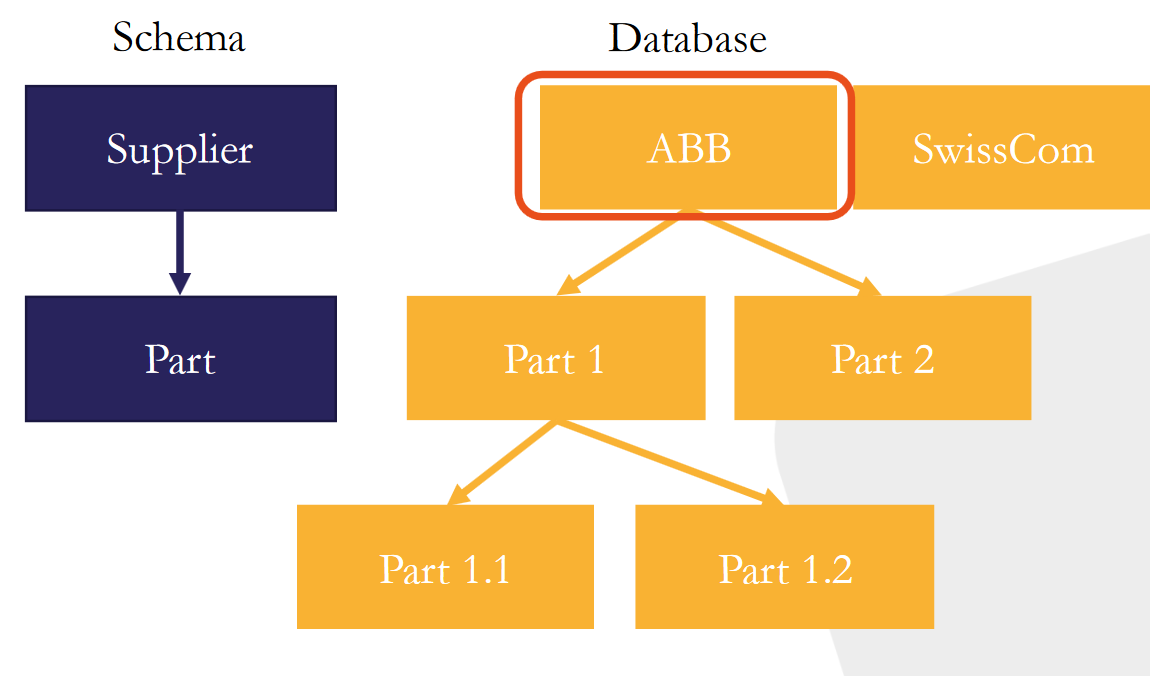
\includegraphics[width=.4\textwidth]{images/IMS.PNG}
\label{IMS_instance}
\caption{IMS Database Schema/Instance}
\end{figure}

\subsection{Network Model}
\begin{figure}[H]
\begin{minipage}[t]{.5\textwidth}
The network model is a data model that organizes its record types not as a tree but as a network instead. Similar to IMS, the query language retrieves one record at a time by doing a traversal on the network, however, they are more natural compared to the hierarchical ones. \\
The network model does not provide data independence or declarative efficient data access, which means it has the same problems as IMS.
\end{minipage}
\begin{minipage}[t]{.5\textwidth}
\strut\vspace*{-\baselineskip}\newline
\centering
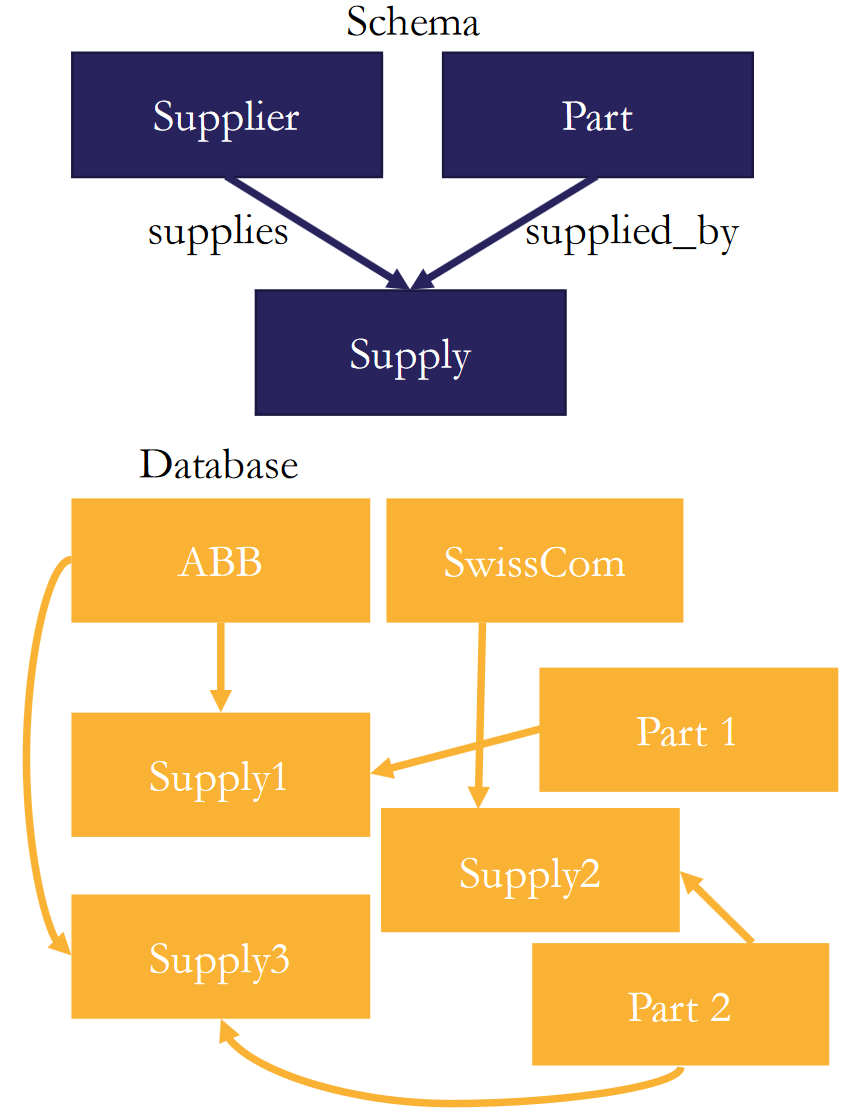
\includegraphics[width=.6\textwidth]{images/Network_Model.PNG}
\label{Network_Model_instance}
\subcaption{Network Model Database Schema/Instance}
\end{minipage}
\end{figure}

\subsection{Relational Model}
The amount of work required to maintain data models that do not offer data independence inspired the relational model. It models the data as a set of relations, where each relation is a set of tuples of the same type. A database scheme is a set of relations and a database instance is a set of instances for each relation. Contrary to the record-at-a-time query languages of IMS and the network model the relational model provides a set-at-a-time query language with support for set operations. \\
The relational model offers both data independence as well as declarative efficient data access. This means the queries do not change on alteration to the data representation since they are declarative and not imperative. Furthermore, this enables automatic query optimization to choose the best execution plan.
\begin{figure}[H]
\centering
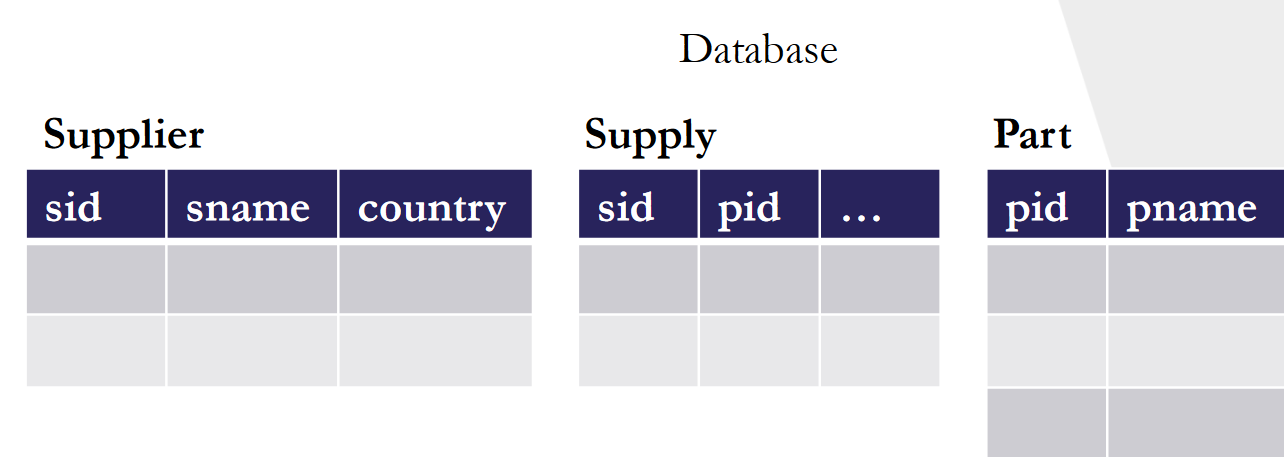
\includegraphics[width=.4\textwidth]{images/Relational_Model_1.PNG}\\
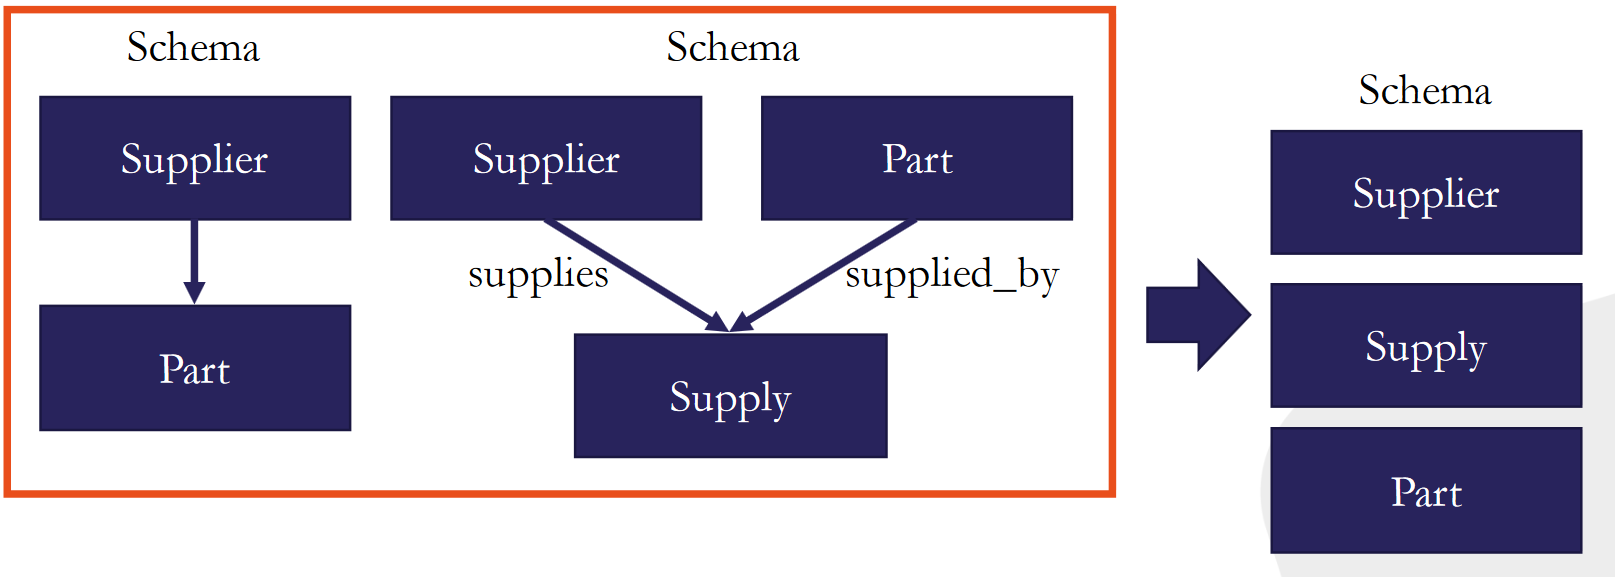
\includegraphics[width=.4\textwidth]{images/Relational_Model_2.PNG}
\label{Relational_Model_instance}
\caption{Relational Model Database Schema/Instance}
\end{figure}

\section{Relational Model, Relational Algebra}
The Relational Model represents data as \textbf{a collection of facts} and inference can be done using \textbf{mathematical logic}. It represents data in the following way:
\begin{itemize}
\item \textbf{Database Schema} - a set of relation schema
\item \textbf{Relation Schema} \begin{itemize}
\item Name
\item A Set of Attributes/Fields/Columns
\end{itemize}
\item \textbf{Field/Attribute} \begin{itemize}
\item Name
\item Domain (e.g., Integer, String)
\end{itemize}
\end{itemize}
\begin{figure}[H]
\centering
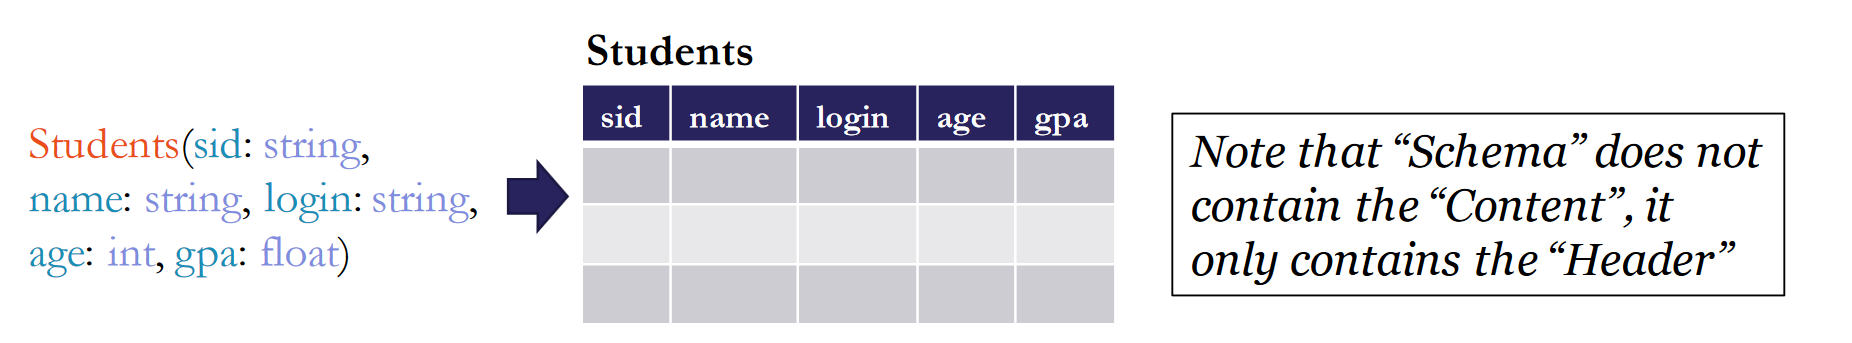
\includegraphics[width=.9\textwidth]{images/schema.PNG}
\label{Relational_Model_schema}
\caption{Example of a Relation Schema}
\end{figure}
Because a relation instance is a \textbf{set}, tuples in the relation are unique and their order does not matter. Real databases might follow a \textbf{bag semantic}, which allows for duplicate tuples. This lecture however will assume \textbf{set semantics} for the relational model.

\subsection{Candidate \& Primary Key}
\textbf{Candidate Key:} The candidate key is a minimal set of fields that identify each tuple uniquely\\
\textbf{Primary Key:} The primary key is a chosen candidate key, which is marked in the relation scheme by underlining \vspace{.2cm}\\
Every relation must have a primary key. Since all relations are sets, it is always possible to find such a key. The \textbf{primary key semantics} are a way to constrain the set of \textit{valid instances}. \\
From a formal point of view; given a relation $R$
\begin{align*}
R(k:D_k, a:D_a, b:D_b)
\end{align*}
with syntax $(attribute\;name : attribute\;domain)$.\\
The set of valid instances $I$ is:
\begin{align*}
I \subseteq D_k \times D_a \times D_b \land \forall(k,a,b), (k', a', b') \in I:\;k = k' \implies (a,b) = (a', b')
\end{align*}

\subsection{Relational Algebra}
One way to query a database modeled in the relational model is called \textbf{relational algebra}. Since relational instances are \textbf{sets} they can be queried \textbf{imperatively} using \textbf{set operations}.

\begin{itemize}
\item \textbf{Union: $\cup$}\\
$x \in R_1 \cup R_2 \iff x \in R_1 \lor x \in R_2$\\
Returns tuples that are in either of the two relations.\\
Union can only be applied if both relations have the same attributes. Since a relation has a \textbf{set of attributes} their order doesn't matter in relational algebra. This means $R(pid, name) \cup S(name, pid)$ is a valid union.
\item  \textbf{Difference: $-$}\\
$x \in R_1 - R_2 \iff x \in R_1 \land \neg(x \in R_2)$\\
Returns tuples that are in the first but not in the second relation.\\
Similar to union, difference can only be applied if both relations share the same attributes.
\item \textbf{Intersection: $\cap$}\\
$R_1 \cap R_2 = R_1 - (R_1 - R_2)$\\
Returns tuples that are in both relations.
\item \textbf{Selection: $\sigma$}\\
$x \in \sigma_c(R) \iff x \in R \land c(x) = True$ where $c$ is a predicate on $R$.\\
Returns tuples that satisfy a given condition.
\item \textbf{Projection: $\Pi_{A_1, ..., A_n}(R)$}\\
Returns only the given attributes of a relation.
\item \textbf{Cartesian Product: $\times$}\\
$(x,y) \in R_1 \times R_2 \iff x \in R_1 \land y \in R_2$\\
Returns all possible combinations of elements in the first and second relation.
\item \textbf{Renaming: $\rho_{B_1, ..., B_n}(R)$}\\
Changes the name of the attributes of $R$ to $B_1, ..., B_n$.
\item \textbf{Natural Join: $\Join$}\\
$R_1(A,B) \Join R_2(C,D) = \Pi_{A,B,C}(\sigma_{R_1.B=R_2.B}(R_1 \times R_2))$\\
Step 1 Selection - check equality on all common attributes\\
Step 2 Projection - eliminate duplicated common attributes\\
Corner Cases: \begin{itemize}
\item No shared attributes: $R \Join S = R \times S$
\item Share all attributes: $R \Join S = R \cap S$
\end{itemize}
\item \textbf{Theta Join: $\Join_\theta$}\\
$R_1 \Join_\theta = \sigma_\theta(R_1 \times R_2)$\\
Joins two relations on a given condition $\theta$.
\item \textbf{Equi-Join: $\Join_{A=B}$}\\
$R_1 \Join_{A=B} R_2 = \sigma_{A=B}(R_1 \times R_2)$\\
Joins two relations on equivalence of two attributes.
\item \textbf{Semi-Join: $\ltimes_c$}\\
$R(A_1, ..., A_n), R_2(B_1, ..., B_n)$\\
$R_1 \ltimes_c R_2 = \Pi_{A_1, ..., A_n}(R_1 \Join_c R_2)$\\
Useful in a trick called \textit{semi-join reduction} for distributed databases.
\item \textit{Relational Division: $\div$}\\
$R \div S = \Pi_{R-S}R - \Pi_{R-S}((\Pi_{R-S}R) \times S - R)$\\
$R \div S = T$ where $T$ is the \textit{largest} relation such that $S \times T \subseteq R$.\\
Only included for completeness, I hate this thing.
\end{itemize}
\begin{figure}[H]
\begin{minipage}[t]{.5\textwidth}
\centering
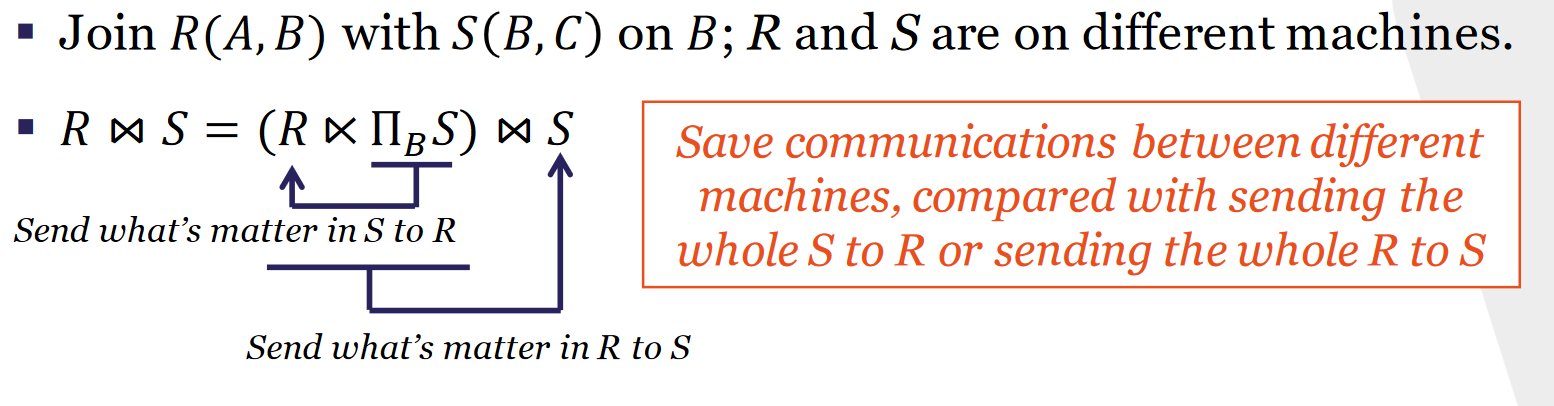
\includegraphics[width=\textwidth]{images/semi-join_reduction.PNG}
\label{semi_join_reduction}
\subcaption{Semi-Join Reduction}
\end{minipage}
\begin{minipage}[t]{.5\textwidth}
\centering
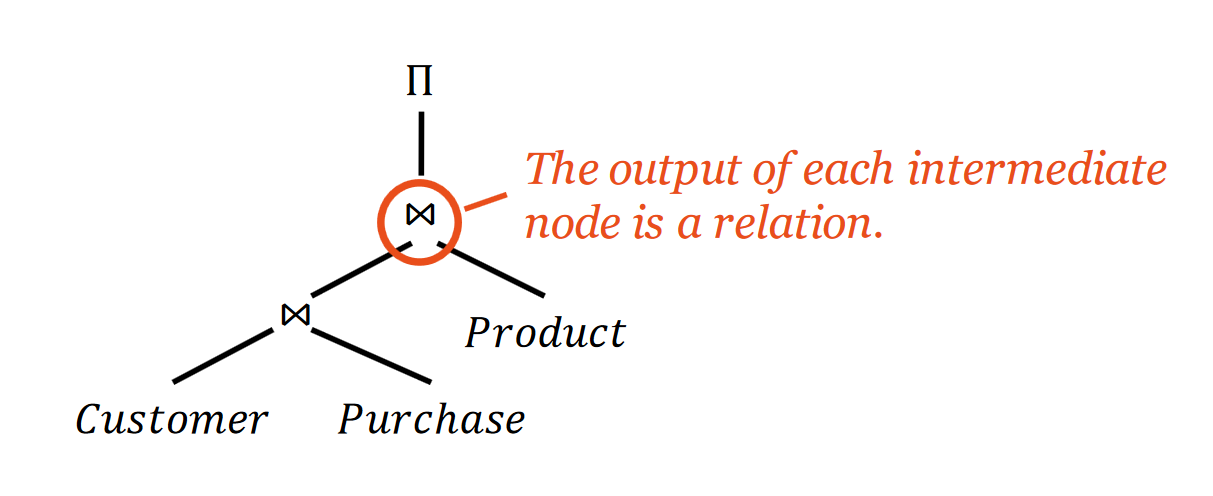
\includegraphics[width=\textwidth]{images/relational_algebra_expression.PNG}
\label{relational_algebra_expression}
\subcaption{Relational Algebra Expression}
\end{minipage}
\end{figure}

It is possible to compose multiple operations together to form a relational algebra expression.
Since relational algebra is not declarative there are different ways to implement the same query. In real world database systems the user does not write relational algebra statements. We hope to have a query language in which the user does not need to worry about different ways of implementing the same thing - we want the system to figure out the optimal way by itself.\vspace{.2cm}\\
One core limitation of relational algebra is the inability to express \textbf{recursion}.

\subsection{Relational Calculus}
Relational calculus takes a different approach than relational algebra. Instead of viewing relations as sets, it considers relations to be \textbf{facts} and queries them using \textbf{first-order logic}.\vspace{.2cm}\\
First-order logic consists of \textbf{syntax} and \textbf{semantics}. The syntax determines which finite sequences of symbols are well-formed expressions in first-order logic, while the semantics determines the meanings behind these expressions. 

\subsubsection{First-Order Logic - Syntax}
The \textbf{alphabet}, i.e. the collection of all legal symbols, is usually divided into \textbf{logical symbols} and \textbf{non-logical symbols}. \\
The logical symbols include the universal and existential quantifiers $\forall$ and $\exists$, the symbols for conjunction $\land$, disjunction $\lor$, implication $\implies$, biconditional $\leftrightarrow$, negation $\neg$ as well as parentheses, brackets, other punctuation symbols, an infinite set of variables, equality symbol $=$ and truth constants $\top$ and $\bot$.\\
The non-logical symbols represent predicates (relations), functions and constants. \\
The formation rules define the terms and formulas of first-order logic. \textbf{Terms} are Variables and Functions (where each argument is a term). A \textbf{formula} can be formed by using predicate symbols, equality, negation, binary connectives and quantifiers. \\
A variable can occur either free or bound. A variable is free, if it is not bound to a quantifier.

\subsubsection{First-Order Logic - Semantics}
The truth value of a formula depends on the \textit{world we live in}. This \textit{world} is semantically defined by the \textbf{interpretation} $\mathbb{I}$. The interpretation determines the \textbf{domain} $\mathbb{D}$, which specifies the range of the quantifiers, and and assigns a set of true tuples of elements to each predicate. \\
A \textbf{model} $\mathcal{M}$ is the tuple $(\mathbb{I}, \mathbb{D}).$ We write
\begin{align*}
\mathcal{M} \models \phi \iff \phi \text{ evaluates to True under } \mathcal{M} \\
\mathcal{M} \not\models \phi \iff \phi \text{ evaluates to False under } \mathcal{M}
\end{align*}
If there are free variables occurring in $\phi$ the truth value depends on the value of the free variables. An \textbf{assignment} maps all free variables to concrete constants. Similarly we write
\begin{align*}
\mathcal{M}, \alpha \models \phi \iff \phi \text{ evaluates to True under } \mathcal{M} \text{ and } \alpha \\
\mathcal{M}, \alpha \not\models \phi \iff \phi \text{ evaluates to False under } \mathcal{M} \text{ and } \alpha
\end{align*}

\subsubsection{Domain Relational Calculus}
Queries in relational calculus can be expressed in a declarative way. It tells the system what we want instead of how to get it. One expresses the query as a set and all tuples belonging to the set are the answer to the query. 
\begin{align*}
\{(pid, cid) \mid \exists n, p (Product(pid, n, p)) \land \exists cn, c (Customer(cid, cn, c)) \land \exists s (Purchase(pid, cid, s))\}
\end{align*}
A formal definition for \textbf{(Domain) Relational Calculus.}
\begin{itemize}
\item Schema
\begin{itemize}
\item Database Schema: $S = (R_1, ..., R_m)$ where each $R_i$ is a Relation.
\item Relation Schema: $R(A_1 : D_1, ..., A_n : D_n)$
\item Domain: $dom = \cup_i D_i$ -- \underline{infinite} set of constants
\end{itemize}
\item Instance
\begin{itemize}
\item Instance of $R(A_1:D_1, ..., A_n:D_n) : I_R \subseteq dom^n$ and $I_R$ is \underline{finite}
\item Instance of DB $S(R_1,...,R_m): \mathbb{I}$ a function that maps $R_i$ to an instance of $R_i$
\end{itemize}
\item An instance of a relation is a finite set of \underline{facts} over the relation
\item An instance of DB is a finite set of \underline{facts} over all relations.
\end{itemize}

Since our domain is infinite it is possible to construct queries in relational calculus that return an \textbf{infinite result}. However, we don't want our database to output infinite answers. Therefore, we classify queries into \textbf{safe queries} and \textbf{unsafe queries}. Let $Q_\phi$ be a relational calculus query. $Q_\phi$ is considered to be \textbf{safe}, if the result $Q_\phi(\mathbb{I})$ is finite for all instances $\mathbb{I}$. 
\begin{figure}[H]
\begin{align*}
\{x \mid \neg R(x)\} \\
\{x \mid \exists y. R(x) \lor R(y)\} \\
\{y \mid \exists x. R(x)\} \\
\{x \mid R(x) \lor \neg R(x)\}
\end{align*}
\caption{Examples of unsafe queries}
\end{figure}
Unfortunately, the problem of deciding whether a query is safe or not is undecidable, since it can be reduced to the satisfiability problem. To get rid of this problem we try to adapt the semantics.

\subsubsection{Domain Independent Relational Calculus}
A query where the answer depends not only on the interpretation of relations (i.e. the database instance) but also on the domain is called \textbf{domain dependent}. We hope to turn a relational calculus query $Q_\phi$ into something domain independent. We define the active domain;
\begin{align*}
adom(Q_\phi, \mathbb{I}) = \text{ all constants in } Q_\phi \text{ and } \mathbb{I}
\end{align*}
From there we define the active domain semantics for $Q_\phi$:
\begin{align*}
Q_{adom(\phi, \mathbb{I})} = \{ (x_1, ..., x_n) \mid \phi \land \forall i, x_i \in adom(\phi, \mathbb{I})\}
\end{align*}
Additionally, all quantifiers $\forall v_i,\; \exists v_i$ in $
Q_\phi$ become $\forall v_i \in adom(\phi, \mathbb{I})$, $\exists v_i \in adom(\phi, \mathbb{I})$. Since both $\phi$ and $\mathbb{I}$ are both finite, a query in relational calculus under active domain semantics will always return a finite answer.
\vspace{.2cm}\\
From a theory side, relational calculus is more powerful than relational algebra, since there are queries that cannot be expressed in relational algebra but can in relational calculus. But Codd's Theorem proves that domain-independent relational calculus is as powerful as relational algebra.\\
Still domain independent relational calculus is still tremendously difficult to analyse.
\begin{itemize}
\item Given a DI-RC query $\phi$, does there exist a DB instance such that it outputs non-empty answers? - \textbf{Satisfiability, undecidable!} 
\item Given two DI-RC queries $\phi_1, \phi_2$, are they equivalent under all possible instances? - \textbf{Equivalence, undecidable!}
\end{itemize}

\subsubsection{Conjunctive Query}
To make the aforementioned properties easier to check we can constrain our query language. 
A conjunctive query has following form:
\begin{align*}
\phi = \exists y_1, ..., y_l (A_1 \land ... \land A_m),\;Q_\phi = \{(x_1, ..., x_n) | \phi \} \text{ each $A_j$ is an atom.}
\end{align*}
Conjective query is as expressive as relational algebra with only selection, projectoin, join and renaming (SPJR Algebra). A one-to-one correspondence in structure can be established \vspace{.1cm}\\
\begin{framed}
\begin{minipage}[t]{.5\textwidth}
\centering
\textbf{\underline{SPJR Algebra}}
\begin{itemize}
\item $R$
\item $\sigma_c(E_1)$
\item $\Pi_{A_1, ..., A_n}(E_1)$
\item $E_1 \times E_2$
\item $\rho_{a_1, ..., a_n}(E_1)$
\end{itemize}
\end{minipage}
\begin{minipage}[t]{.5\textwidth}
\centering
\textbf{\underline{Conjunctive Query}}
\begin{itemize}
\item $\{x \mid R(x)\}$
\item $\{x \mid \phi_{E_1}(x) \land \phi_c(x)\}$
\item $\{(x_1, ..., x_n)\; |$\\$\;  \exists o_1, ..., o_k.\;\phi_{E_1} (x_1, ..., x_n, o_1, ..., o_k)\}$
\item $\{(x,y) \mid \phi_{E_1}(x) \land \phi_{E_2}(y)\}$
\end{itemize}
\end{minipage}
\end{framed}

\begin{figure}[H]
\centering
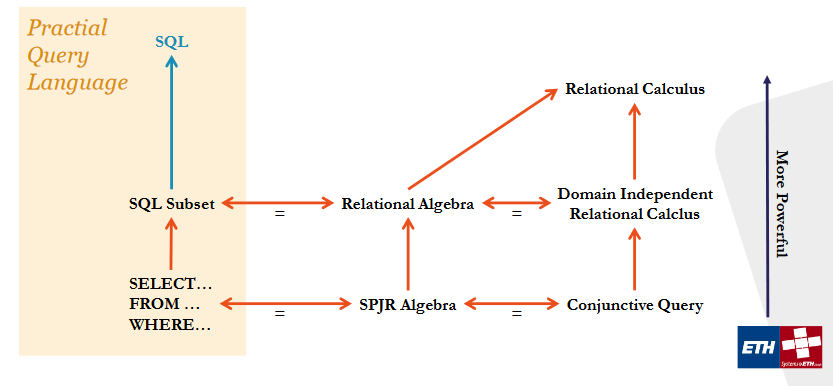
\includegraphics[width=.9\textwidth]{images/language_power.PNG}
\caption{Expressiveness of Languages in Comparison}
\label{Language_power}
\end{figure}

\section{Structured Query Language}
SQL is a family of standards consisting of
\begin{itemize}
\item Data Definition Language (DDL)
\item Data Manipulation Language (DML)
\item Query Language
\end{itemize}
It is important to note that contrary to relational calculus and relational algebra SQL relations \textbf{have bag semantics.}

\subsection{Data Definition Language (DDL)}
The data definition language provides statements to define the relation schema. In the relational model a relation schema looks like $R(f_1 : D_1, ..., f_n : D_n)$. In SQL the schema is defined by providing the \textbf{relation name, a set of attributes and their types}.

\subsubsection{Table Basics}
A table in a relational database is defined by it's name and columns. The number, type and order of columns is fixed and each column has a name. The data type of the column constrains the set of possible values that can be assigned to a column. \\
A table is created by the \textit{CREATE TABLE} command. In this command one specifies the name of the table, the name of the columns and their respective datatype. For example;
\begin{lstlisting}[language=SQL] 
CREATE TABLE products (
	pid integer,
	name text,
	price numeric
);
\end{lstlisting}
Similarly a table can be deleted using the \textit{DROP TABLE} command.
\begin{lstlisting}[language=SQL]
DROP TABLE products;
\end{lstlisting}

\subsubsection{Default Values}
A column can be assigned a default value. When a new row is created and no values are specified for some columns, those columns will be filled with their respective default values. If no default value is declared specifically, the default value is the null value.
\begin{lstlisting}[language=SQL]
CREATE TABLE products (
	pid SERIAL,
	name text,
	price numeric DEFAULT 420.69,
	buy_time timestamp CURRENT_TIMESTAMP
);
\end{lstlisting}
Common default values are \textit{SERIAL}, which is a shortcut to supply successive values or \textit{CURRENT\_TIMESTAMP} to provide the timestamp at the time of insertion.

\subsubsection{Constraints}
A \textbf{primary key constraint} indicates that a column, or a group of columns, can be used as a unique identifier for rows in the table. This requires that the values are both \textbf{unique and not null}. \vspace{.2cm}\\
\begin{minipage}{.5\textwidth}
\begin{lstlisting}[language=SQL]
CREATE TABLE products (
	pid integer PRIMARY KEY,
	name text,
	price numeric,
	buy_time timestamp
);
\end{lstlisting}
\end{minipage}\hfill
\begin{minipage}{.45\textwidth}
\begin{lstlisting}[language=SQL]
CREATE TABLE example (
	a integer,
	b integer,
	c integer,
	PRIMARY KEY (a, c)
);
\end{lstlisting}
\end{minipage}

\subsubsection{Modifying Tables}
When requirements of the application change or mistakes have been made it is very easy to drop a table and create it again. However, this is not a convenient option if the table is already filled with data, or if the table is referenced by other database objects (for instance a foreign key constraint). Postgresql provides a family of commands to make modifications to existing tables. This is conceptually different to altering data contained in the table; here we alter the definition of the relation schema. All operations are performed using the \textit{ALTER TABLE} command.\vspace{.1cm}
\begin{addmargin}{-.5cm}
\begin{itemize}
\item \textbf{Add/Remove Columns}
\begin{lstlisting}[language=SQL]
ALTER TABLE products ADD COLUMN description text;
ALTER TABLE products DROP COLUMN description;
ALTER TABLE products ADD COLUMN description text CHECK (description <> '');
ALTER TABLE products DROP COLUMN description CASCADE;
\end{lstlisting}
When creating a new column, it is initially filled with whatever default value is given. If no default value is specified the column is filled with null. Additionally, all options for columns can also be applied (i.e. default values, constraints). 
\item \textbf{Add/Remove Constraints}
\begin{lstlisting}[language=SQL]
ALTER TABLE products ADD CHECK (name <> '');
ALTER TABLE products ADD CONSTRAINT some_name UNIQUE (product_no);
ALTER TABLE products ADD FOREIGN KEY (product_group_id) REFERENCES product_groups;
ALTER TABLE products ALTER COLUMN product_no SET NOT NULL;
\end{lstlisting}
To add a not-null constraint, which cannot be written as a table constraint, the above syntax is used. This constraint will be checked immediately, so the table data must satisfy the constraint before it can be added.\\
To remove a constraint you need to know its name. If you know the name it is easy. Otherwise the system assigned a generated name, which can be found out with \textit{\\d tablename}.As with dropping a column, you need to add \textit{CASCADE} if you want to drop a constraint that something else depends on. An example is that a foreign key constraint depends on a unique or primary key constraint on the referenced columns. It works the same for all constraint types except not-null constraints. To drop a not-null constraint the syntax below can be used.
\begin{lstlisting}[language=SQL]
ALTER TABLE products DROP CONSTRAINT some_name;
ALTER TABLE products ALTER COLUMN product_no DROP NOT NULL;
\end{lstlisting}
\item \textbf{Change/Remove Default Values}
\begin{lstlisting}[language=SQL]
ALTER TABLE products ALTER COLUMN price SET DEFAULT 6.9;
ALTER TABLE products ALTER COLUMN price DROP DEFAULT;
\end{lstlisting}
Changing the default value does not affect any existing tuples in the table, it just changes the default for future \textit{INSERT} commands. Removing a default value is essentially the same as setting it to the null value. Dropping a default that does not exist hence does not produce an error.
\item \textbf{Change Column Data Types}
\begin{lstlisting}[language=SQL]
ALTER TABLE products ALTER COLUMN price TYPE numeric(10,2);
\end{lstlisting}
Changing a columns data type will only succeed if the existing entries can be converted to the new type by an implicit cast. For more complex casts the \textit{USING} clause can be used to specify how to compute the new values. Postgres will try to convert the column's default values and constraints that involve the column to the new type. These conversions might fail or produce surprising results. It is often best to drop any constraints on the column before conversion.
\item \textbf{Rename Columns/Tables}
\begin{lstlisting}[language=SQL]
ALTER TABLE products RENAME COLUMN product_no TO pid;
ALTER TABLE products RENAME TO items;
\end{lstlisting}
\end{itemize}
\end{addmargin}

\subsection{Data Manipulation Language (DML)}
\subsubsection{Inserting Data}
A new tuple can be created using the \textit{INSERT} command. The command requires the table name and the column values.
\begin{lstlisting}[language=SQL]
INSERT INTO products VALUES (1, 'Cheese', 9.99);
\end{lstlisting}
The data values are listed in the order in which the columns are defined in the table, separated by commas. The data values are either literals or scalar expressions. To avoid the need to know the order of the columns, the columns can be listed explicitly.
\begin{lstlisting}[language=SQL]
INSERT INTO products (product_no, name, price) VALUES (1, 'Cheese', 9.99);
\end{lstlisting}
If not all columns of the table are stated, the columns are filled from the left with as many values as are given and the rest of the columns assumes their default value. It is also possible to request the default value explicitly using the \textit{DEFAULT} keyword. It is also possible to insert multiple rows in a single statement or insert the result of a query, which may return one or several tuples.
\begin{lstlisting}[language=SQL]
INSERT INTO products (product_no, name, price) VALUES
	(1, 'Cheese', 9.99),
	(2, 'Bread', 1.99);
INSERT INTO products (product_no, name, price)
	SELECT product_no, name, price FROM new_products
		WHERE release_date = 'today';
\end{lstlisting}

\subsubsection{Updating Data}
Existing rows can be updated via the \textit{UPDATE} command, which requires three pieces of information.
\begin{enumerate}
\item The name of the table and column to be updated
\item The new value of the column
\item Which rows to update
\end{enumerate}
Since SQL does generally not provide a unique identifier for each row, rows are identified by whether they specify a given condition. Only if there is a primary key, specified or not, individual rows can be addressed. An update command will try to update all rows that fulfil the given condition, which may be zero, one or multiple rows. It does not produce an error to attempt an update that does not match any rows. If multiple columns need to be updated they are separated by commas.
\begin{lstlisting}[language=SQL]
UPDATE products SET price = 10 where price = 5;
UPDATE mytable SET a = 5, b = 3, c = 1 WHERE a > 0;
\end{lstlisting}

\subsubsection{Deleting Data}
Similarly to updating rows, rows are deleted based on whether they match a given condition, since generally rows cannot be addressed individually. Rows are deleted using the adequately named \textbf{DELETE} command.
\begin{lstlisting}[language=SQL]
DELETE FROM products WHERE price = 10;
\end{lstlisting}
Simply stating a table name will delete all rows in said table!
\begin{lstlisting}[language=SQL]
DELETE FROM products;
\end{lstlisting}

\subsubsection{Returning Data from Modified Rows}
Sometimes it is useful to obtain data from modified rows while they are being manipulated. The \textit{INSERT}, \textit{UPDATE}, and \textit{DELETE} commands all have an optional \textit{RETURNING} clause supporting this. The allowed contents of a \textit{RETURNING} clause are the same as a \textit{SELECT} command's output list. It can contain column names, or value expressions using those columns. In an \textit{INSERT} command the rows are returned as they were inserted. In an \textit{UPDATE} statement, the returned data is the content of the modified row. In a \textit{DELETE} command the content of the deleted rows is returned.
\begin{lstlisting}[language=SQL]
CREATE TABLE users (firstname text, lastname text, id SERIAL PRIMARY KEY);
INSERT INTO users (firstname, lastname) VALUES ('Joe', 'Cole') RETURNING id;

UPDATE products SET price = price * 1.1
	WHERE price <= 99.99
	RETURNING name, price AS new_price
DELTE FROM products WHERE obsoletion_date = 'today'
	RETURNING *;	
\end{lstlisting}

\subsubsection{Snapshot Semantics}\
How does SQL deal with this?
\begin{lstlisting}[language=SQL]
DELETE FORM requires WHERE prerequisite IN 
(SELECT follow-up FROM requires);
\end{lstlisting}
SQL conducts the \textit{DELETE} in two phases.
\begin{itemize}
\item \textbf{Phase 1:} {\color{orange} Mark} all tuples which are affected by the updates.
\item \textbf{Phase 2:} {\color{NavyBlue} Implement} updates on the marked tuples.
\end{itemize}
Mixing the two phases would lead to non-deterministic results.
\begin{figure}[H]
\centering
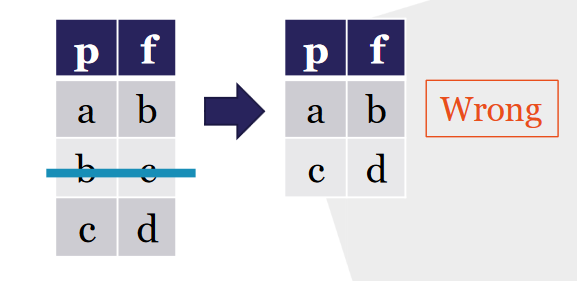
\includegraphics[width=.4\textwidth]{images/snapshot_semantics.PNG}
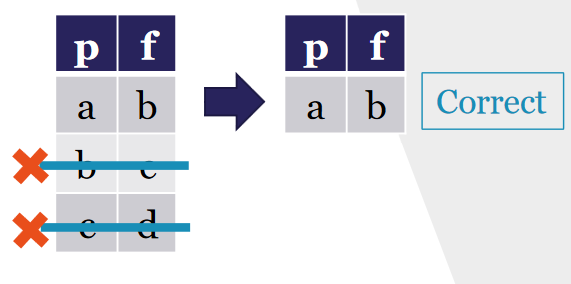
\includegraphics[width=.4\textwidth]{images/snapshot_semantics2.PNG}
\caption{Incorrect and Correct Outcome}
\label{snapshot_semantics}
\end{figure}

\subsection{Query Language}
In SQL the \textit{SELECT} command is used to specify queries. The general syntax of the \textit{SELECT} command is;
\begin{lstlisting}[language=SQL]
[WITH with_queries] SELECT select_list FROM table_expression [sort_specification]
\end{lstlisting}

\subsubsection{Table Expressions}
A table expression computes a table. The table expression contains a \textit{FROM} clause that is optionally followed by \textit{WHERE}, \textit{GROUP BY,} and \textit{HAVING} clauses. \vspace{.2cm}\\
\begin{addmargin}{-.5cm}
\begin{itemize}
\item \textbf{The FROM Clause}
The \textit{FROM} clause derives a table from one or more other tables given in a comma-separated table reference list.
\begin{lstlisting}[language=SQL]
FROM table_reference [, table_reference [, ...]]
\end{lstlisting}
A table reference can be a table name or a derived table such as a subquery, a \textit{JOIN} construct, or a complex combination of these. \textbf{If more than one table reference is listed in the \textit{FROM} clause, the tables are cross-joined}.

\item \textbf{Joined Tables}
A joined table is a table derived from two other (real or derived) tables according to the rules of the particular join type. Inner, outer, and cross-joins are available. The general syntax is:
\begin{lstlisting}[language=SQL]
T1 join_type T2 [ join_condition ]
\end{lstlisting}
Joins of all types can be chained together, or nested. Either or both T1 and T2 can be joined tables. Parentheses can be used around join clauses to control the join order. In absence of parentheses the order is left-to-right.\vspace{.2cm}\\
\textbf{Cross Join}
\begin{lstlisting}[language=SQL]
T1 CROSS JOIN T2
\end{lstlisting}
The cross join is a Cartesian product. It takes all possible combinations of rows from T1 and T2 and appends them in the joined table.\vspace{.2cm}\\
\textbf{Qualified Joins}
\begin{lstlisting}[language=SQL]
T1 { [INNER] | { LEFT | RIGHT | FULL } [OUTER] } JOIN T2 ON boolean_expression
T1 { [INNER] | { LEFT | RIGHT | FULL } [OUTER] } JOIN T2 USING ( join column list )
T1 NATURAL { [INNER] | {LEFT | RIGHT | FULL } [OUTER] } JOIN T2
\end{lstlisting}
Above is the general syntax of a qualified join. \textit{INNER} and \textit{OUTER} are optional in all forms. The default is \textit{INNER} and \textit{LEFT, RIGHT,} and \textit{FULL} imply an outer join. The join condition is specified in the \textit{ON} or \textit{USING} clause, or implicitly by \textit{NATURAL.}\vspace{.2cm}\\
\textbf{Inner Join}\\
Logically, a cross join is performed and each pair of rows that does not satisfy the condition is removed.\vspace{.2cm}\\
\textbf{Left Outer Join}\\
An inner join is performed. Then for each row in T1 that does not match the condition with any row from T2 (,i.e. is not in the joined table of the inner join), a joined row is added with null values for the columns in T2.\vspace{.2cm}\\
\textbf{Right Outer Join}\\
Same principle as a left outer join but the tables are reversed. For each row in T2 that does not match the condition with any row from T1, a joined row is added with null values for the columns in T1.\vspace{.2cm}\\
\textbf{Full Outer Join}\\
Same principle as left/right outer join but joined rows are added for rows from both tables that do not match the condition.\vspace{.2cm}\\
\textbf{ON Clause}\\
The \textit{ON} clause takes a boolean expression of the same kind that is used in a \textit{WHERE} clause. A pair of rows matches the \textit{ON} clause if the expression evaluates to true.\vspace{.2cm}\\
\textbf{USING Clause}\\
The \textit{USING} clause is a shorthand for an equality check on columns. It takes a comma-separated list of shared column names and creates a join condition that includes an equality comparison for each one. The following join conditions are the same.
\begin{lstlisting}[language=SQL]
T1 JOIN T2 USING (a, b);
T1 JOIN T2 ON T1.a = T2.a AND T1.b = T2.b;
\end{lstlisting}
Additionally, the output of \textit{JOIN USING} suppresses redundant columns.\vspace{.2cm}\\
\textbf{Natural}\\
\textit{NATURAL} is a shorthand form of \textit{USING} that includes all column names that appear in both tables. If there are no common columns it behaves like a cross-join.
\item \textbf{Table And Column Aliases}\\
A temporary name can be given to tables and complex table references to be used in the rest of the query. This is called a table alias. A table alias can be created using the following syntax.
\begin{lstlisting}[language=SQL]
FROM table_reference AS alias
FROM table_reference alias
\end{lstlisting}
A common application is to assign a short identifier to long table names to keep clauses readable. The alias becomes the new name of the table and the \textbf{original name cannot be used in the query.} Aliases are necessary in self-joins and if the table reference is a subquery.\\
It is also possible to alias the columns of the table as well as the table itself. If fewer column aliases are supplied than the table has columns, the remaining columns are not named.
\begin{lstlisting}[language=SQL]
FROM table_reference [AS] alias ( column1 [, column2 [, ...]] )
\end{lstlisting}
\item \textbf{Subqueries}\\
Subqueries specifying a derived table must be enclosed in parentheses and must be assigned a table alias.
\begin{lstlisting}[language=SQL]
FROM (SELECT * FROM table1) AS alias_name
\end{lstlisting}
\item \textbf{The WHERE Clause}\\
After processing of the \textit{FROM} clause, each row of the derived table is checked against the search condition. If the result of the condition is true, the row is kept in the output table. 
\item \textbf{The GROUP BY and HAVING Clauses}\\
After passing the \textit{WHERE} filter, the derived input table can be grouped using \textit{GROUP BY} and groups can be eliminated using the \textit{HAVING} clause.
\begin{lstlisting}[language=SQL]
SELECT select_list
	FROM ...
	[WHERE ...]
	GROUP BY grouping_column_reference [, grouping column_reference]...
	HAVING boolean_expression
\end{lstlisting}
\end{itemize}
\end{addmargin}

\subsubsection{Distinct}
Duplicate results in the output can be eliminated using the \textit{DISTINCT} key word. It is written directly after the \textit{SELECT}. The key word \textit{ALL} can be used to specify the default behaviour of retaining all rows. Null values are considered equal in comparison. An arbitrary condition of equality can be specified using \textit{DISTINCT ON}.
\begin{lstlisting}[language=SQL]
SELECT DISTINCT select_list ...
SELECT ALL select_list ... %default behaviour
SELECT DISTINCT ON (expression) select_list ...
\end{lstlisting}

\subsubsection{Combining Queries}
The result of two queries can be combined using the set operations union, intersection and difference. The syntax is
\begin{lstlisting}[language=SQL]
query1 UNION [ALL] query2
query1 INTERSECT [ALL] query2
query EXCEPT [ALL] query2
\end{lstlisting}
To use any of the three operations, the two queries must be "union compatible", which means that they return the same number of columns and the corresponding columns have compatible data types.
\begin{itemize}
\item \textbf{Union}\\
\textit{UNION} appends all results of query2 to the result of query1. Additionally, it \textbf{eliminates duplicates} unless \textit{UNION ALL} is used.
\item \textbf{Intersect}\\
\textit{INTERSECT} returns all rows that are both in the result of query1 and query2. Duplicate rows are eliminated unless \textit{INTERSECT ALL} is used.
\item \textbf{Except}\\
\textit{EXCEPT} returns all rows that are in the result of query1 but not in the result of query2. Duplicate rows are eliminated unless \textit{EXCEPT ALL} is used.
\end{itemize}

\subsubsection{Sorting Rows}
A query will return the rows in an arbitrary order. With the \textit{ORDER BY} clause it is possible to specify how the rows should be ordered. The sort expression(s) can be any expression that would be valid in the query's select list. When more than one expression is specified, the later values are used to sort rows that are equal according to the earlier values.
\begin{lstlisting}[language=SQL]
SELECT select_list FROM table_expression
	ORDER BY sort_expression1 [ASC | DESC] [NULLS { FIRST | LAST }]
\end{lstlisting}
The key words \textit{ASC} and \textit{DESC} determine whether the rows are sorted ascending or descending, with ascending being the default. \textit{NULLS FIRST/LAST} options can be used to choose whether null values should appear before or after non-null values in the order. \textit{NULLS FIRST} is the default for \textit{DESC} order, and \textit{NULLS LAST} otherwise.

\subsubsection{Subquery Expressions}
\begin{itemize}
\item \textbf{Exists}
The arguments of \textit{EXISTS} is an arbitrary \textit{SELECT} statement, or subquery. The subquery is evaluated to determine whether it returns any rows. If it returns at least one row, the result of \textit{EXISTS} is true. If the subquery returns no rows, the result is false. The subquery is usually only run until the result is clear, therefore no queries with side effects should be used.
\begin{lstlisting}[language=SQL]
EXISTS (subquery)
\end{lstlisting}
\item \textbf{In}
\begin{lstlisting}[language=SQL]
expression IN (subquery)
\end{lstlisting}
The right-hand side is a parenthesized subquery, which must return exactly one column. The left-hand expression is evaluated and compared to each row of the subquery result. The result of \textit{IN} is true if any equal subquery row is found. The result is false if no matching row is found. \\
If the left-hand expression returns null or if there are no equal right-hand values and at least one right-hand row is null the result of the \textit{IN} construct is null not false.
\item \textbf{Not In}
\begin{lstlisting}[language=SQL]
expression NOT IN (subquery)
\end{lstlisting}
Analogous to \textit{IN}. The result of \textit{NOT IN} is true if only unequal subquery rows are found and false if an equal row is found. 
\item \textbf{Any/Some}
\begin{lstlisting}[language=SQL]
expression operator ANY (subquery)
expression operator SOME (subquery)
\end{lstlisting}
The left-hand expression is evaluated and compared to each row of the subquery result using the given operator, which must yield a boolean result. The result of \textit{ANY} is true if any true result is obtained and false otherwise. \textit{SOME} is a synonym for \textit{ANY}.
\item \textbf{All}
\begin{lstlisting}[language=SQL]
expression operator ALL (subquery)
\end{lstlisting}
The left-hand expression is evaluated and compared to each row of the subquery result using the given operator, which must yield a boolean result. The result of \textit{ALL} is true if all rows yield true. The result is false if any false results are found. The result is null if no comparison with a subquery returns false, and at least one comparison returns null.
\end{itemize}

\section{Known, Unknowns, and Views}
So far we have assumed that all information in a relation is complete, but in practice we often have incomplete information in our database. This can happen if something is not applicable or the data is simply missing.

\subsection{Null}
One way to model incomplete information is to replace the values that we do not know with a special state \textbf{null}. It is important to mention that \textit{NULL} is a state, not a value. A null value introduces a lot of corner cases for many operations. A few are listed below;
\begin{itemize}
\item Arithmetic \begin{itemize}
\item $(NULL + 2) \to NULL$
\item $(NULL *0) \to NULL$
\end{itemize}
\item Comparisons\begin{itemize}
\item $NULL = NULL \to Unknown$
\item $(NULL < 13) \to Unknown$
\item $(NULL > NULL) \to Unknown$
\end{itemize}
\item 3-value Logic\vspace{.2cm}\\
\begin{minipage}[t]{.3\textwidth}
\begin{tabular}{|l|l|}
\hline
\textbf{not} &            \\ \hline
true         & false     \\ \hline
unknown      & unknown  \\ \hline
false        & true     \\ \hline
\end{tabular}
\end{minipage}
\begin{minipage}[t]{.3\textwidth}
\begin{tabular}{|l|l|l|l|}
\hline
\textbf{and} & true & unknown & false \\ \hline
true & true & unknown & false \\ \hline
unknown & unknown & unknown & false \\ \hline
false & false & false & false \\ \hline
\end{tabular}\vspace{.2cm}\\
\begin{tabular}{|l|l|l|l|}
\hline
\textbf{or} & true & unknown & false \\ \hline
true & true & true & true \\ \hline
unknown & true & unknown & unknown \\ \hline
false & true & unknown & false \\ \hline
\end{tabular}
\end{minipage}
\item State not Value\begin{itemize}
\item $(NULL = NULL) \to Unknown$
\item $(NULL\;IS\;NULL) \to Unknown$
\end{itemize}
\item Null in Aggregations \begin{itemize}
\item Null in \textit{GROUP BY} - all nulls form a single group
\item Null in Values - Most operators will ignore the NULL value (count(*) will not)
\end{itemize}
\end{itemize}
Null can come appear in various contexts. One being \textit{INSERT} commands where for some columns no value is supplied. Another example are outer joins.
\begin{figure}[H]
\centering
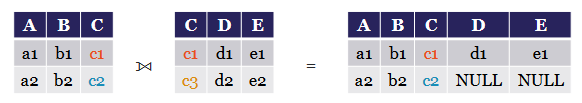
\includegraphics[width=.8\textwidth]{images/outer_join_introducing_null.PNG}
\caption{Left Outer Join Introducing Null}
\label{join_introducing_null}
\end{figure}

\subsubsection{View}
A relation is a powerful abstraction that provides us with \textit{physical data independence.} A view aims at raising the level of abstraction even higher, and provide us with \textit{logical data independence}, i.e. the user can use view without caring about how relations are organized underneath the cover. \\
In a database, a view is the result set of a stored query on the data, which the database users can query just as they would in a persistent database collection object. 
\begin{figure}[H]
\centering
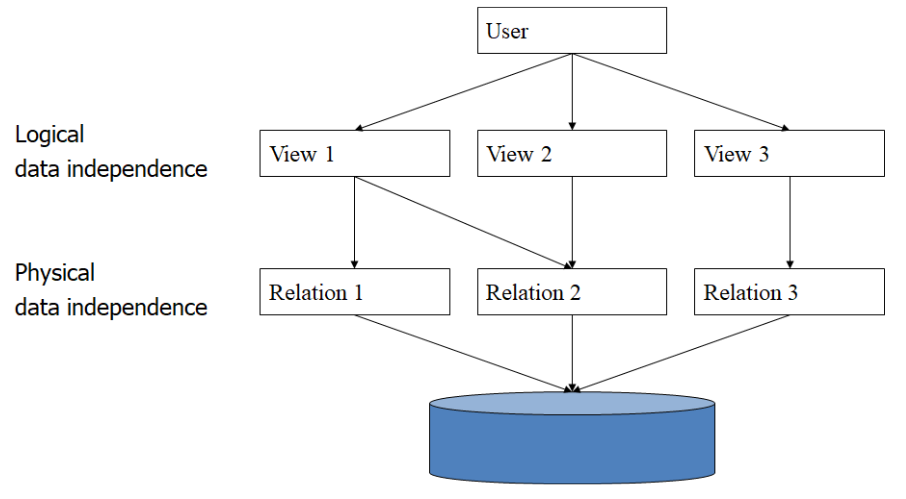
\includegraphics[width=.5\textwidth]{images/view_independence.PNG}
\label{view_independence}
\caption{Logical and Physical Data Independence}
\end{figure}
A view can be created using the \textit{CREATE} command.
\begin{lstlisting}[language=SQL]
CREATE VIEW name_of_view AS (subuery);
\end{lstlisting}
Then the view can be used just like a table, even if it logically has never been materialized. Views have several different applications:
\begin{itemize}
\item \textbf{Privacy}\\
A view can be used for access control and preserving privacy. A user who has access to a relation, knows all the information in said table. A user who only has access to the view, only knows the information that is present in the view.
\item \textbf{Usability}\\
A view can be used to make writing some queries easier. It is essentially like a named subquery. It may not look like a big saving but in practice the saving can be significant. Views make the queries a lot more readable.
\item \textbf{Is-a-Relationship}\\
A view can be used to implement generalization. 
\begin{figure}[H]
\centering
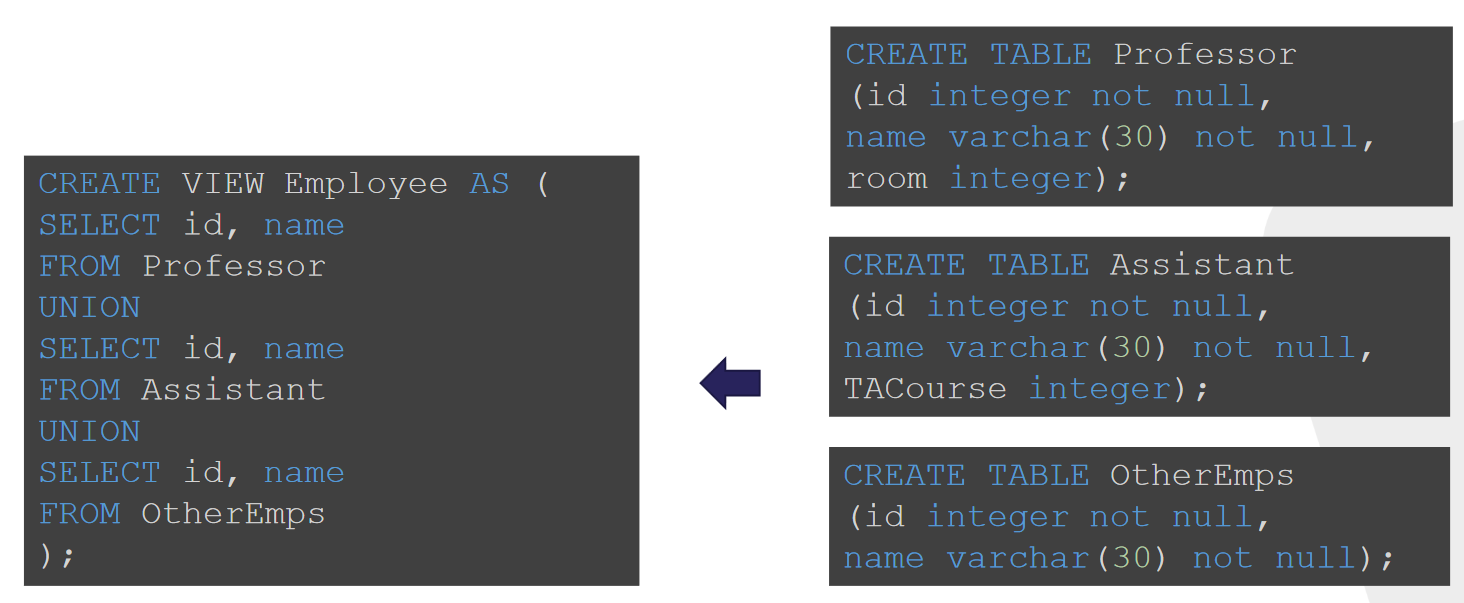
\includegraphics[width=.8\textwidth]{images/view_generalization.PNG}
\label{view_generalization}
\caption{Generalization using View}
\end{figure}
\end{itemize}
A view gets evaluated by query rewriting. First the view is replaced by its defining query and then optimized by the database management system.\vspace{.3cm}\\

Is it possible to update a view? First we have to define what that means exactly. Assuming there are base relations $R_1, ..., R_n$ and a view $V = Q(R_1, ..., R_n)$ defined over these relations. \\
If the user wants to update $V$ into $V'$, the task is to find a set of updates to the base relation $R_1', ..., R_n'$ such that $Q(R_1',...,R_n') = V'$. It is not always possible to find such updates. Following are a few examples of views, that are not updateable.
\begin{figure}[H]
\begin{minipage}[t]{.5\textwidth}
\centering
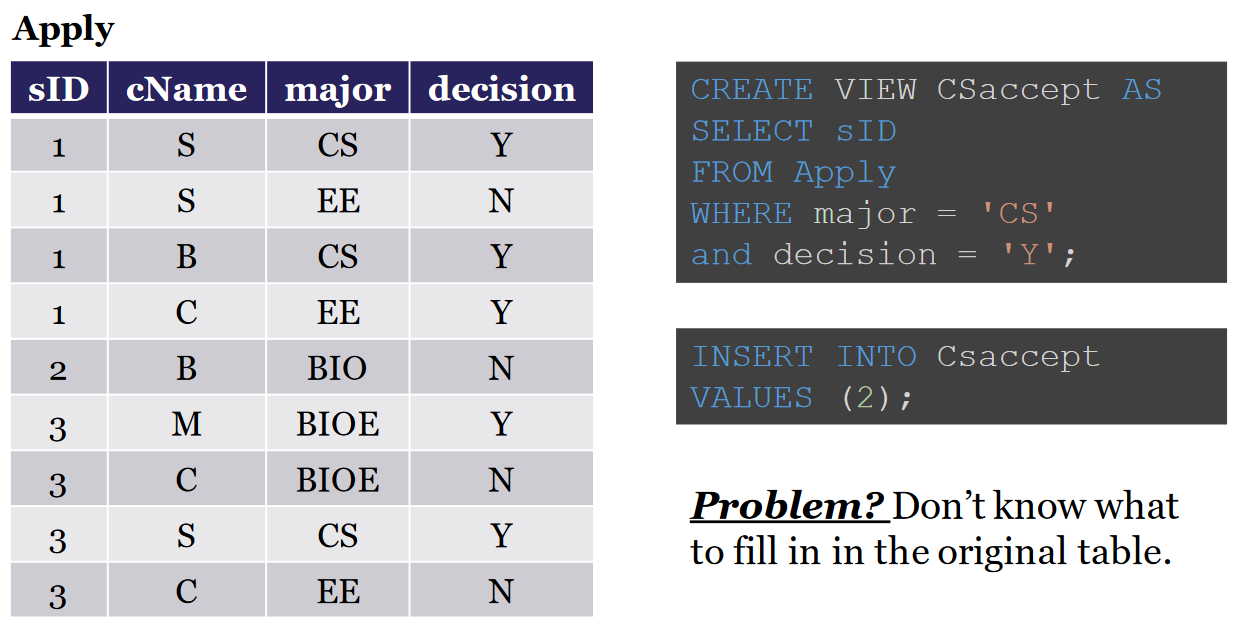
\includegraphics[width=.97\textwidth]{images/projection_update.PNG}
\label{projection_update}
\subcaption{Non updatable Projection View}
\end{minipage}
\begin{minipage}[t]{.5\textwidth}
\centering
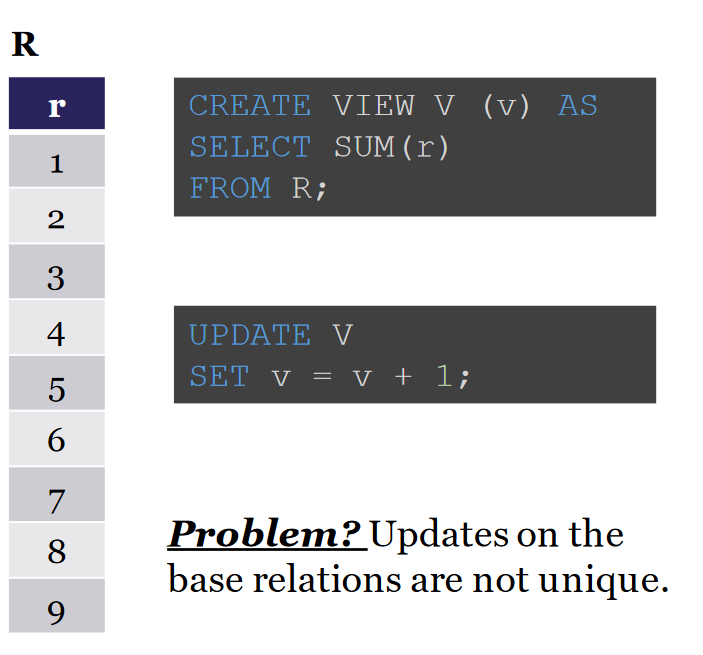
\includegraphics[width=.6\textwidth]{images/aggregation_view.PNG}
\label{aggregation_view}
\subcaption{Non updatable Aggregation View}
\end{minipage}
\end{figure}
\noindent But it is not all bad news. There also exist views that are easier to update.
\begin{figure}[H]
\centering
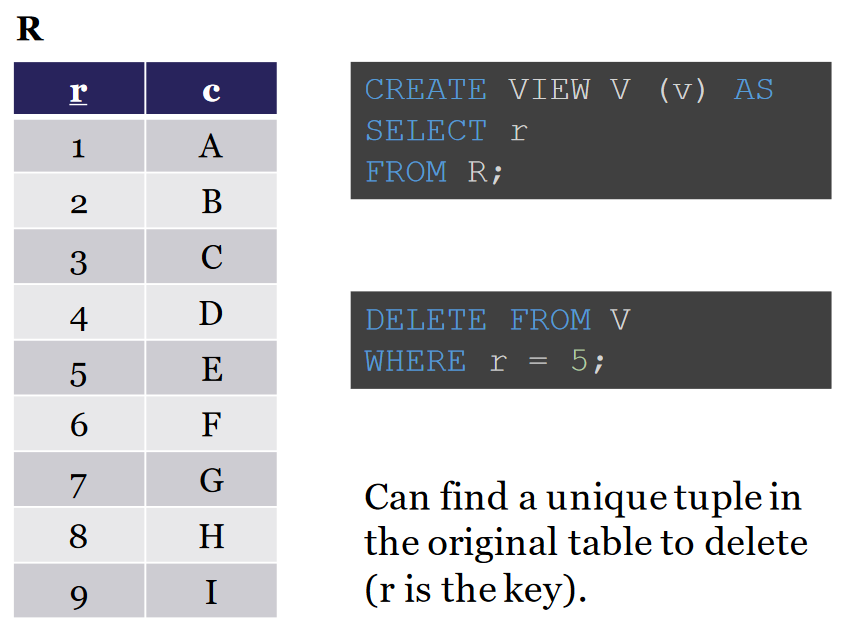
\includegraphics[width=.5\textwidth]{images/updatable_view.PNG}
\label{updatable_view}
\caption{Updatable View}
\end{figure}
\begin{figure}[H]
\begin{minipage}{.5\textwidth}
\begin{itemize}
\item Principle:
\begin{itemize}
\item SQL tries to avid indeterminism.
\item SQL is conservative with view updates.
\end{itemize}
\item A SQL view is updatable if and only if:
\begin{itemize}
\item The view involves only ONE base relation.
\item The view involves the key of that base relation.
\item The view does NOT involve aggregates, group by, or duplicate-elimination.
\end{itemize}
\item What's the intuition of these three rules?
\begin{itemize}
\item Try to maintain one-to-one mapping between the view and the base relation
\end{itemize}
\end{itemize}
\end{minipage}
\begin{minipage}{.5\textwidth}
\centering
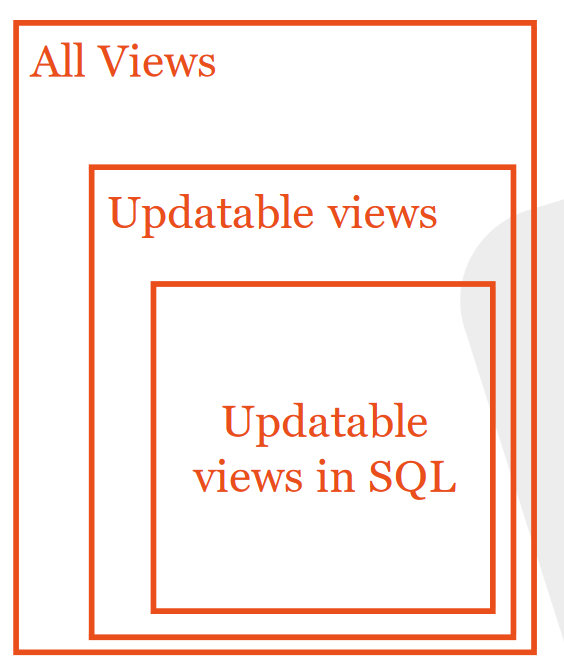
\includegraphics[width=.8\textwidth]{images/views.PNG}
\subcaption{Hierarchy of Views}
\label{views}
\end{minipage}
\end{figure}

\section{Recursion and Integrity Constraints}
\subsection{Recursion}
Recursion provides the functionality to execute the same query again and again until it converges.
\begin{lstlisting}[language=SQL]
WITH RECURSIVE R as
(base query)
UNION
(recursive query)
<Query involving R and other tables>
\end{lstlisting}
Recursion can be tricky and lead to non terminating queries. Since recursion is mostly used to determine the transitive closure over graphs, it makes sense to look into graph databases when the workload contains a lot of recursion queries.

\subsection{Integrity Constraints}
Constraints define the set of valid database instances.
\subsubsection{Not Null Constraint}
The values of a certain attribute cannot be null.
\begin{lstlisting}[language=SQL]
CREATE TABLE student (
	sID int,
	sName text,
	GPA real not null);
\end{lstlisting}

\subsubsection{Primary Key Constraint}
The attributes need to be unique and not null.
\begin{lstlisting}[language=SQL]
CREATE TABLE student (
	sID int PRIMARY KEY,
	sName text,
	GPA real);
\end{lstlisting}
A primary key can be defined over multiple attributes but there can only be one primary key per relation. The combination needs to be unique and no attribute can be null.
\begin{lstlisting}[language=SQL]
CREATE TABLE students (
	sID int,
	sName text,
	GPA real
	PRIMARY KEY (sID, sName));
\end{lstlisting}

\subsubsection{Unique Constraint}
A certain attribute needs to be unique. It is possible to define multiple unique constraints for one relation, which can be over one or several attributes. Unique columns may have multiple null rows.
\begin{lstlisting}[language=SQL]
CREATE TABLE student (
	sID int UNIQUE,
	sName text,
	GPA real
	UNIQUE (sID, sName)
	UNIQUE (sID, GPA));
\end{lstlisting}

\subsubsection{Check Constraint}
\textit{CHECK} constraints can be used to conduct local value checking of attributes. Check constraints only reject false tuples, unknown and true are accepted.
\begin{lstlisting}[language=SQL]
CREATE TABLE student (
	sID int,
	sName text,
	semester int,
	GPA real
	check(GPA + semester = 10));
\end{lstlisting}

\subsubsection{Referential Constraint}
Foreign keys refer to tuples from a different relation. The attribute cannot take a value that does not exist in the referenced table or it has to be null.
\begin{lstlisting}[language=SQL]
CREATE TABLE R (
a integer PRIMARY KEY, b varchar(3) UNIQUE);

CREATE TABLE S (...,
	ka integer references R);
\end{lstlisting}

\subsubsection{Referential Constraints: Maintenance}
What happens if we delete a row that is referenced in another table? This is problematic because referenced values have to exist. There are different options to handle this case;
\begin{itemize}
\item \textbf{Cascade}\\
Propagate update or delete
\item \textbf{Restrict}\\
Prevent deletion of the primary key before trying to do the change, cause an error
\item \textbf{No Action}\\
Prevent modifications after attempting the change, cause an error
\item \textbf{Set default, set null}\\
Set references to null or a default value.
\end{itemize}
\begin{figure}[H]
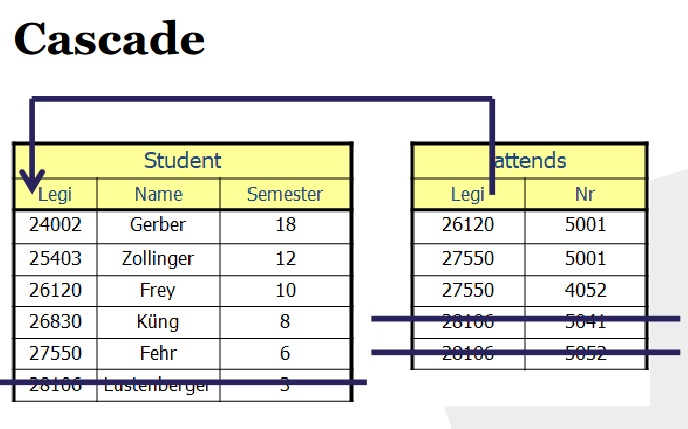
\includegraphics[width=.5\textwidth]{images/cascade.PNG}
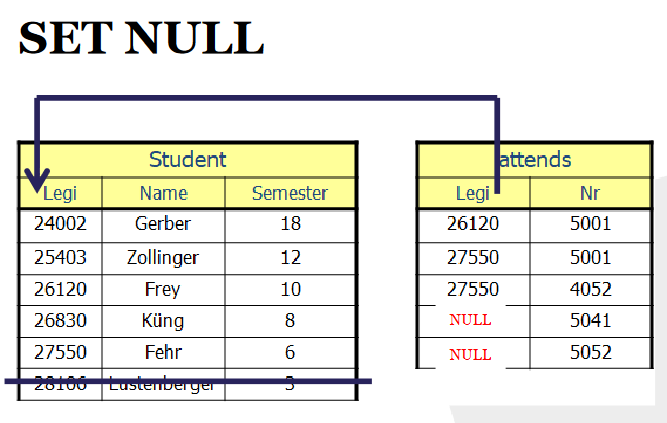
\includegraphics[width=.5\textwidth]{images/set-null.PNG}\\
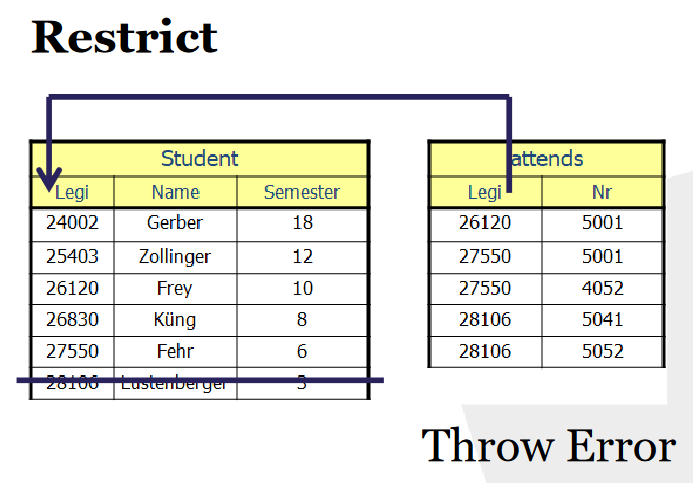
\includegraphics[width=.5\textwidth]{images/restrict.PNG}
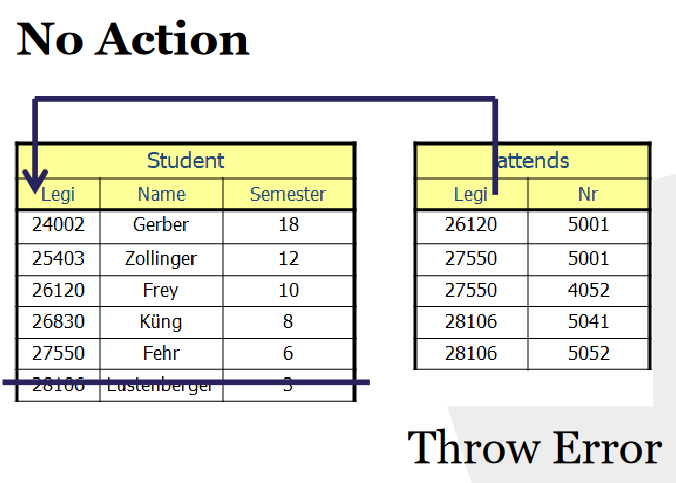
\includegraphics[width=.5\textwidth]{images/no-action.PNG}
\caption{Update Modes}
\label{update_modes}
\end{figure}
The difference between restrict and no action is very subtle and in many database management systems there is no difference at all. In principle, restrict throws an error immediately while no action throws an error after trying.

\section{Entity-Relationship Model}
The process of implementing a real-world application contains the following steps:
\begin{figure}[H]
\centering
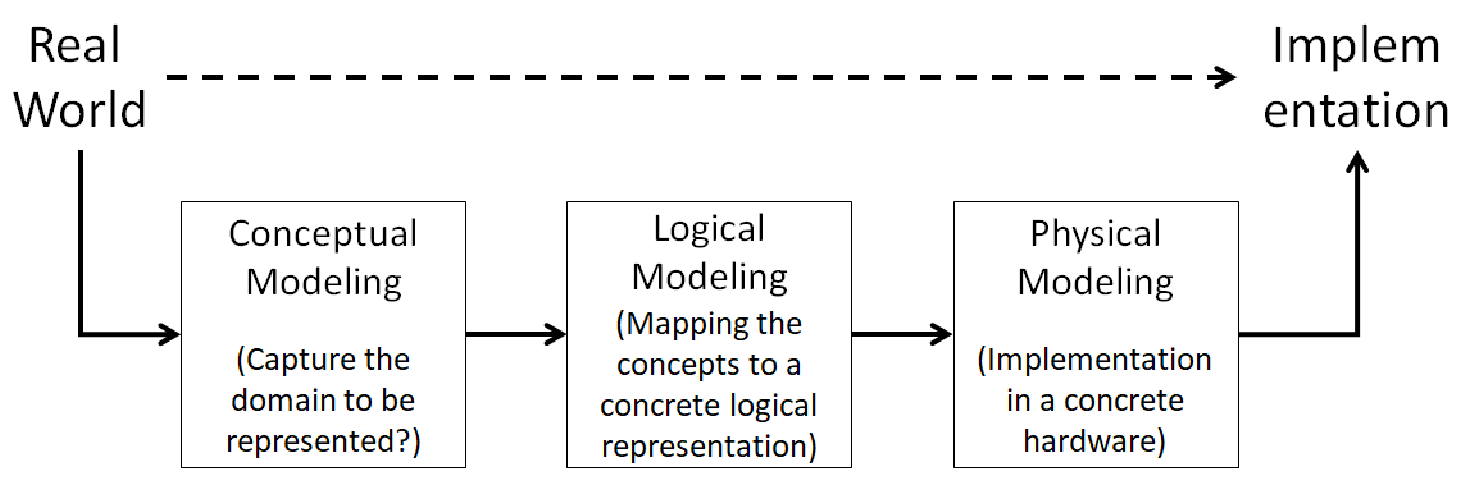
\includegraphics[width=.8\textwidth]{images/implementation.PNG}
\label{implementation}
\caption{Modeling Process}
\end{figure}
Conceptual modeling tries to capture the domain to be represented. It only contains elements that are explicitly stated and not things that seem like common sense. The logical modeling converts the conceptual model into a logical representation, which is then concretely implemented by the physical modeling.\\
The conceptual model specifies all valid instances. \vspace{.3cm}\\

\noindent One way of conceptual modeling is the creation of an \textbf{entity-relationship model}. An ER model, models an application in the following three element types:
\begin{itemize}
\item \textbf{Entity Sets}
\begin{itemize}
\item A set of similar entities
\item Entity: An object in the real world that is distinguishable from other objects
\item "Similar": Entities in the same entity set share the same attributes
\item Roughly equivalent to classes in object-oriented programming
\end{itemize}
\item \textbf{Attributes}
\item \textbf{Relationships}
\begin{itemize}
\item Relationships are connections among two or more entity sets.
\end{itemize}
\end{itemize}
An ER-diagram is a graphical way of representing entities and the relationships among them.
\begin{figure}[H]
\centering
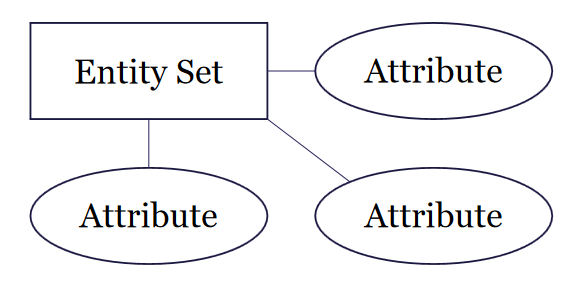
\includegraphics[width=.4\textwidth]{images/entity_set.PNG}
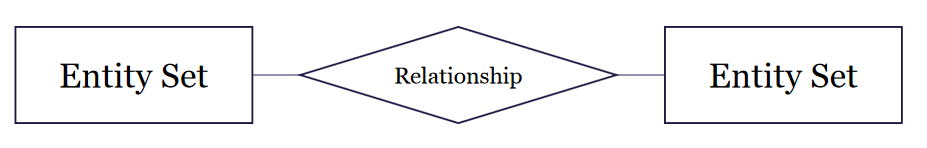
\includegraphics[width=.5\textwidth]{images/relationships.PNG}
\label{er_diagram}
\caption{Entity-Relationship Diagram}
\end{figure}
\subsection{Keys}
A key is a minimal set of attributes whose values uniquely identify an entity in the set. There might be multiple keys, all of them are called candidate keys. Only one candidate key is called the primary key and it is underlined in the schema. Each identity set must have a primary key.

\subsection{Formal Semantics}
ER-diagrams are a graphical way of modeling data, but that does not make them vague or imprecise. ER-diagrams can be made formal by defining a mapping from an ER-diagram to a set of database instances.
\begin{itemize}
\item All values we can take $\mathcal{D} = \mathcal{B} \cup \Delta$
\begin{itemize}
\item Concrete Values (Int, String, Floating Point, etc.): $\mathcal{B}$
\item Abstract Values (Corresponding to an entity): $\Delta$
\end{itemize}
\item Entity Set $E \implies$ 1-ary Predicate $E(x)$. [$E(x) = True$ if $x$ is of Entity Type $E$]
\item Attribute $A \implies$ binary Predicate $A(x,y)$. [$A(x,y) = True$ if $x$ has attribute $y$]
\item n-ary Relation $R \implies$ n-ary Predicate $R(x_1, ..., x_n)$. [$R(x_1, ..., x_n) = True$ if $(x_1, ..., x_n)$ participate in $R$]
\item A first-order interpretation $\mathcal{J}$ satisfies:
\begin{itemize}
\item $E^\mathcal{J} \subseteq \Delta$
\item $A^\mathcal{J} \subseteq \Delta \times \mathcal{B}$
\item $R^\mathcal{J} \subseteq \Delta^n$
\end{itemize}
\end{itemize}
Each subgraph introduces a first-order logic sentence. This tells us what a valid database instance should satisfy. A relationship is simply a type constraint.
\begin{figure}[H]
\begin{minipage}[t]{.5\textwidth}
\centering
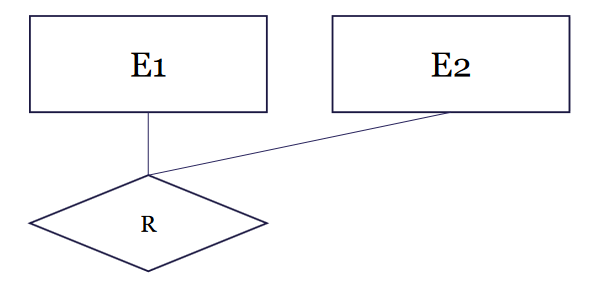
\includegraphics[width=\textwidth]{images/diagram_logic.PNG}
\label{diagram_logic}
\begin{align*}
\forall x_1 \in \Delta, x_2 \in \Delta.\; R(x_1, x_2) \implies E_1(x_1) \land E_2(x_2)
\end{align*}
\end{minipage}
\begin{minipage}[t]{.5\textwidth}
\centering
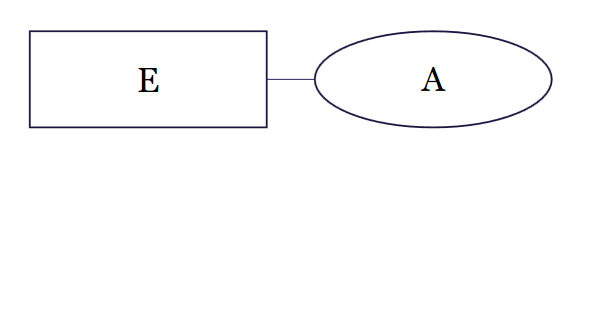
\includegraphics[width=\textwidth]{images/entity_logic.PNG}
\label{entity_logic}
\begin{align*}
\forall x, E(x)\implies \exists !\;y.\;A(x,y) \land y \in \mathcal{B}.
\end{align*}
\end{minipage}
\caption{Entity-Relation Introducing Logic Constraints}
\end{figure}
Checking whether two ER-diagrams are equivalent comes down to checking whether the first-order logic sentences are equivalent.

\subsection{Cardinality}
\begin{itemize}
\item \textbf{1-to-many relationship} - A is in a 1-to-may relationship with B if one A entity can have relationship with multiple B entities, and one B entity can only have relationship with only one A entity.
\begin{figure}[H]
\centering
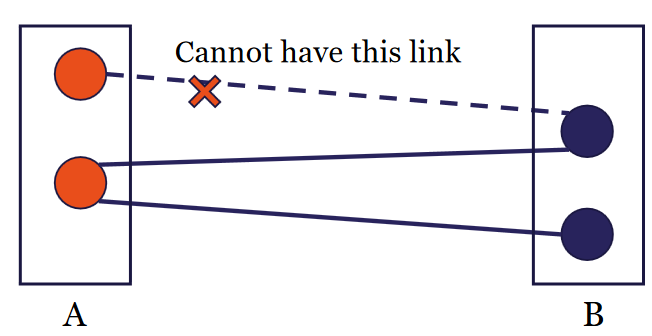
\includegraphics[width=.45\textwidth]{images/1-to-many1.PNG}
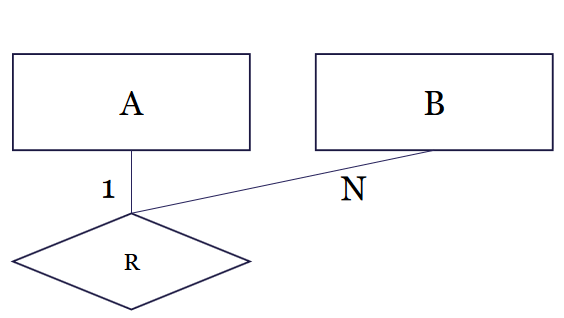
\includegraphics[width=.5\textwidth]{images/1-to-many2.PNG}
\label{1-to-many}
\caption{1-to-many Relationship}
\end{figure}
\item \textbf{many-to-1 relationship} - A is in a many-to-1 relationship with B if one B entity can have relationship with multiple A entities, and one A entity can only have relationship with only one B entity.
\begin{figure}[H]
\centering
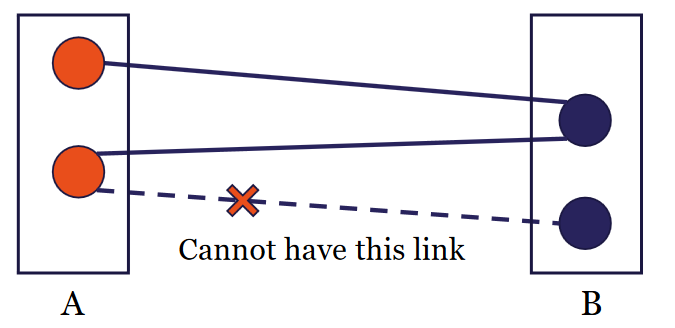
\includegraphics[width=.45\textwidth]{images/many-to-one1.PNG}
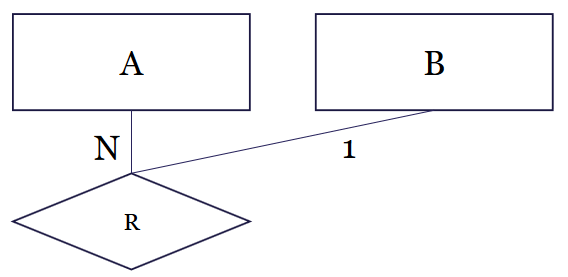
\includegraphics[width=.5\textwidth]{images/many-to-one2.PNG}
\label{many-to-1}
\caption{many-to-1 Relationship}
\end{figure}
\item \textbf{1-to-1 relationship} - A is in a 1-to-1 relationship with B if one A entity can only have relationship with one B entity, and one B entity can only have relationship with one A entity.
\begin{figure}[H]
\centering
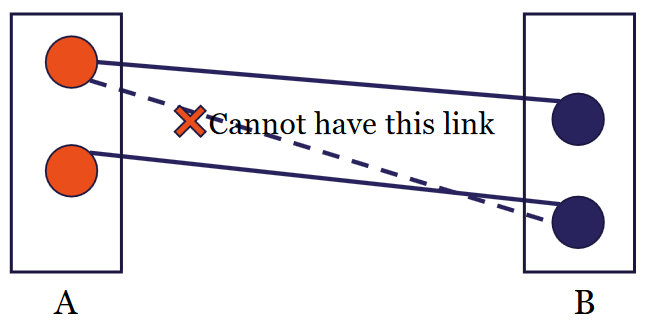
\includegraphics[width=.45\textwidth]{images/one-to-one1.PNG}
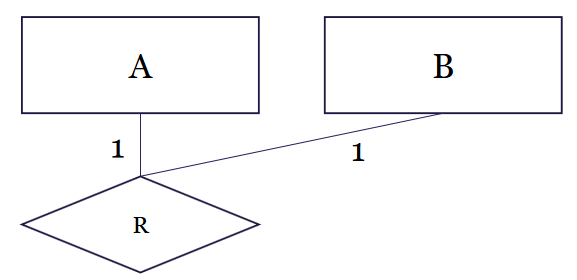
\includegraphics[width=.5\textwidth]{images/one-to-one2.PNG}
\label{1-to-1}
\caption{1-to-1 Relationship}
\end{figure}
\item \textbf{many-to-many relationship} - A is in a many-to-many relationship with B if one A entity can have relationships with multiple B entities, and one B entity can have relationships with multiple A entity.
\begin{figure}[H]
\centering
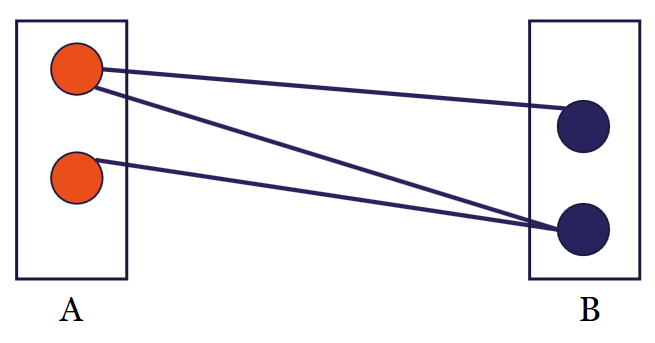
\includegraphics[width=.45\textwidth]{images/many-to-many1.PNG}
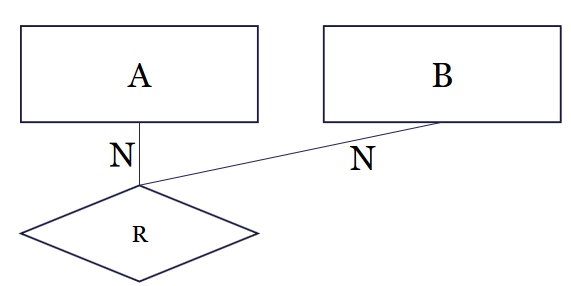
\includegraphics[width=.5\textwidth]{images/many-to-many2.PNG}
\label{many-to-many}
\caption{many-to-many Relationship}
\end{figure}
\end{itemize}
Every "1" in the diagram is associated with a first-order logic constraint.
\begin{figure}[H]
\begin{minipage}{.5\textwidth}
The ER-diagram on the right specifies the following two constraints:
\begin{itemize}
\item $\forall x_A, x_B, x_C, x_D.\; R(x_A, x_B, x_C, x_D) \implies$\\
$\neg\exists x_A'.\;R(x_A', x_B, x_C, x_D) \land (x_A' \neq x_A)$
\item $\forall x_A, x_B, x_C, x_D.\; R(x_A, x_B, x_C, x_D) \implies$\\
$\neg\exists x_C'.\;R(x_A, x_B, x_C', x_D) \land (x_C' \neq x_C)$
\end{itemize}
\end{minipage}
\begin{minipage}{.5\textwidth}
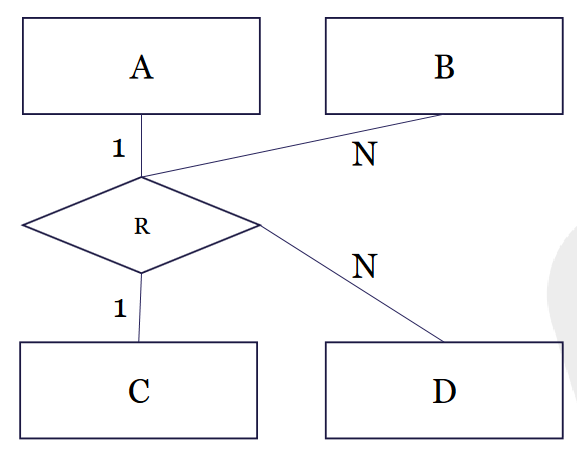
\includegraphics[width=.8\textwidth]{images/cardinality.PNG}
\end{minipage}
\end{figure}
\noindent We can also have a more expressive (min, max)-notation.
\begin{figure}[H]
\begin{minipage}{.6\textwidth}
This specifies the following constraints:
\begin{itemize}
\item $\forall x_A.\;A(x_A) \implies$\\$ \exists^{\geq a_{min},\leq a_{max}} x_B',x_C'.\;R(x_A, x_B', x_C')$
\item $\forall x_B.\;B(x_B) \implies$\\$ \exists^{\geq b_{min},\leq b_{max}} x_A',x_C'.\;R(x_A', x_B, x_C')$
\item $\forall x_C.\;C(x_C) \implies$\\$ \exists^{\geq c_{min},\leq c_{max}} x_A',x_B'.\;R(x_A', x_B', x_C)$
\end{itemize}
\end{minipage}
\begin{minipage}{.4\textwidth}
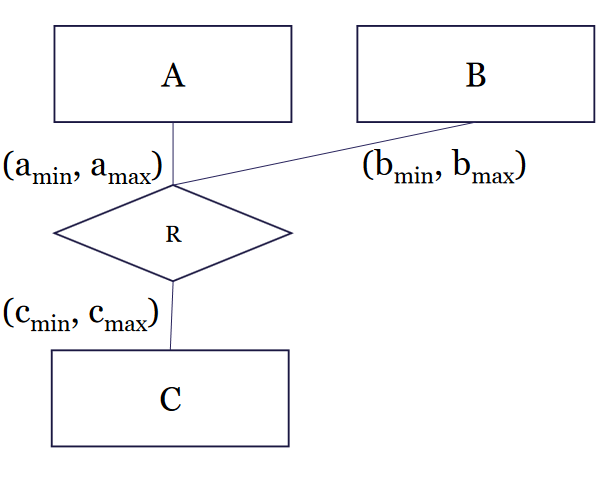
\includegraphics[width=\textwidth]{images/expressive_cardinality.PNG}
\end{minipage}
\end{figure}

\subsection{Weak Entity}
Some entity's existence relies on other entries. For example a room cannot exist without a building. This means room is a weak entity relying on building. The key of room is therefore \underline{(Bld\#, Room\#)}. 

\subsection{Generalization}
Generalization are "is-a" relationships. This means that the entities share the generalized attributes (and primary key). For example both a professor and a student are people and therefore share people attributes.
\begin{figure}[H]
\begin{minipage}[t]{.5\textwidth}
\centering
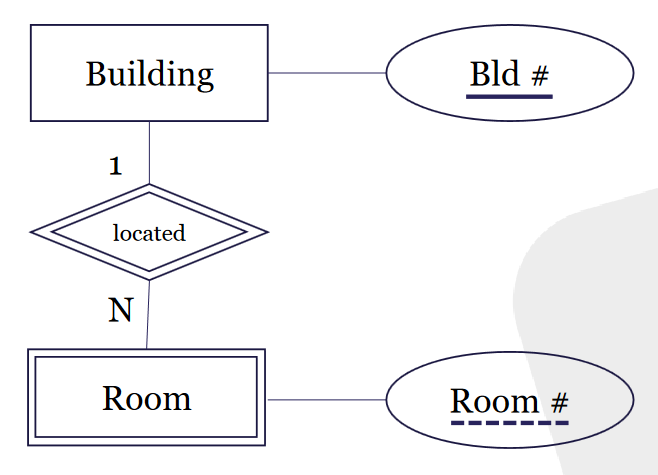
\includegraphics[width=.8\textwidth]{images/weak_entity.PNG}
\label{weak_entity}
\subcaption{Weak Entity}
\end{minipage}
\begin{minipage}[t]{.5\textwidth}
\centering
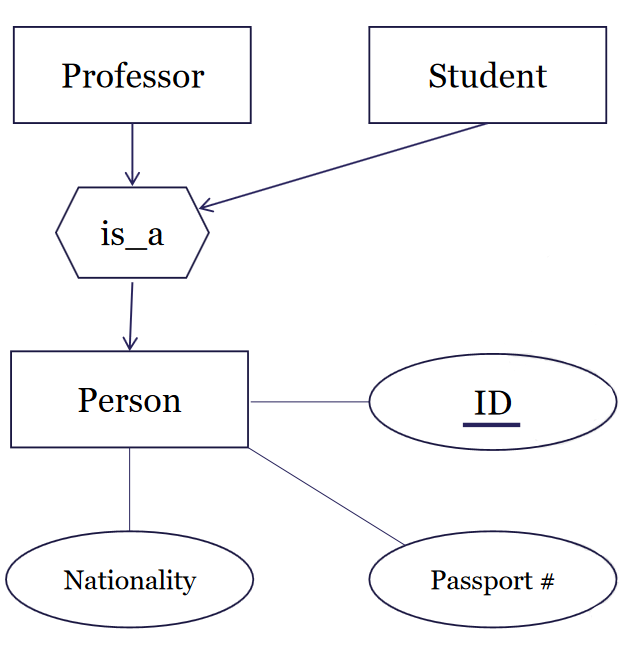
\includegraphics[width=.8\textwidth]{images/generalization.PNG}
\label{generalization}
\subcaption{Generalization}
\end{minipage}
\end{figure}

\subsection{ER-Model to Relational Model}
If we have conceptually modeled our application in the entity-relationship model, we can logically model it in the relational model. The following principles apply to the conversion.
\begin{itemize}
\item Entities become relations.
\item Relationships become relations.
\item Merge relations with the same key.
\item Generalization.
\item Weak entities.
\item entity sets become tables.
\item attributes of entity sets become attributes of the table.
\item When there are no cardinality constraints, relationships become tables, containing the keys of all participating entity sets.
\end{itemize}

\section{Functional Dependency}
A badly designed database will experience a list of problems.
\begin{itemize}
\item Update-Anomaly
\item Insert-Anomaly
\item Delete-Anomaly
\end{itemize}

\subsection{Redundancy}
One of the causes for such anomalies can be redundancy. It is a waste of storage space and it incurs additional work to keep multiple copies of data consistent. However redundancy is not always bad. Through redundancy it is possible to improve locality. It is a tradeoff between space and performance. Sometimes redundancy is even needed for example to provide fault tolerance and ensure availability.\\
No matter whether redundancy is good or bad, we want to understand:
\begin{itemize}
\item How to \textit{model} data redundancy?
\item How to \textit{reason} about redundancy?
\end{itemize}
The notion on how to do this is called \textbf{functional dependency}.
\vspace{.4cm}\\
Given\begin{itemize}
\item Schema: Relation e.g. $\mathcal{R}(A:D_A, B:D_B, C:D_C, D:D_D)$
\item Instance: $R\subseteq D_A \times D_B \times D_C \times D_D$
\item Let $\alpha \subseteq \mathcal{R}, \beta \subseteq \mathcal{R}$\\
$\alpha$ is a subset of attributes.
\end{itemize}
There exists a \textbf{functional dependency} $\alpha \to \beta$ if and only if $\forall r, s \in R:\;r.\alpha = s.\alpha \implies r.\beta = s.\beta$. In other words, there exists a functional dependency $\alpha \to \beta$ if and only if for any two tuples $r$ and $s$ in database instance $R$, if $r$ and $s$ share the same value on columns $\alpha$, then they share the same values on column $\beta$. \\
We write $R \models \alpha \to \beta$ if $R$ satisfies $\alpha \to \beta$.

\subsubsection{Keys \& Cardinalities}
\begin{itemize}
\item $\alpha \subseteq R$ is a superkey iff
\begin{itemize}
\item $a \to \mathcal{R}$ ($\mathcal{R}$ means all columns)
\item This means that if we know the value of columns $\alpha$, we know the value for the rest of the columns in $\mathcal{R}$. $\implies \alpha$ must be a superset of a key.
\end{itemize}
\item $\alpha \to \beta$ is minimal iff
\begin{itemize}
\item $\forall A \in \alpha:\; (\alpha - \{A\} \not\to \beta$
\end{itemize}
\item Notation for minimal functional dependencies:
\begin{itemize}
\item $\alpha \dot{\to} \beta$
\end{itemize}
\item $\alpha \subseteq \mathcal{R}$ is a candidate key iff
\begin{itemize}
\item $\alpha \dot{\to} \mathcal{R}$
\end{itemize}
\end{itemize}
There also exists a relationship between keys and cardinalities.
\begin{itemize}
\item Cardinalities define functional dependencies
\item Functional dependencies determine keys
\item Not all functional dependencies are derived from the cardinality information.
\end{itemize}

\subsubsection{Inference}
Assuming we are given a set of functional dependencies $F$. We want to figure out how new functional dependencies can be \textit{implied} from this set of functional dependencies. There are two ways to define which functional dependencies will follow:
\begin{itemize}
\item $F \models \alpha \to \beta$: Semantics - Any $R$ that satisfies $F$ will also satisfy $\alpha \to \beta$
\item $F \vdash \alpha \to \beta$: Syntax - We can derive $\alpha \to \beta$ by applying a set of inference rules over $F$.
More precisely:
\begin{itemize}
\item Let $F$ be a set of FDs on scheme $\mathcal{R}$ and $\alpha \to \beta$ be another FD on $\mathcal{R}$. Then $F$ implies $\alpha \to \beta$, denoted by $F \models \alpha \to \beta$, if every relation instance $R$ of $\mathcal{R}$ that satisfies all FDs in $F$ also satisfies $\alpha \to \beta$.
\item Let $F$ be a set of FDs on scheme $\mathcal{R}$. Then, the \textbf{closure} of $F$, denoted by $F^+$, is the set of all FDs implied by $F$.
\item Let $F$ and $G$ be sets of FDs on scheme $\mathcal{R}$. Then $F$, and $G$ are \textbf{equivalent}, denoted by $F \equiv G$, if $F \models G$ and $G \models F$.
\end{itemize}
\end{itemize}
A fundamental result shows that inference by syntax and inference by semantics are equivalent.
\begin{align*}
F \models \alpha \to \beta \iff F \vdash \alpha \to \beta. \text{ when $\vdash$ is defined by Armstrong's Axioms)}
\end{align*}
Armstrong's axioms provide us with inference rules:
\begin{itemize}
\item \textbf{Reflexivity}
\begin{itemize}
\item $\alpha \subseteq \beta \implies \beta \to \alpha$
\item Special case: $\mathcal{R} \to \alpha$
\item We call these FDs \textbf{trivial FDs}.
\end{itemize}
\item \textbf{Augmentation}
\begin{itemize}
\item $\alpha \to \beta \implies \alpha\gamma \to \beta\gamma$
\item (Notation $\alpha\gamma := \alpha \cup \gamma$)
\end{itemize}
\item \textbf{Transitivity}
\begin{itemize}
\item $\alpha \to \beta \land \beta \to \gamma \implies \alpha \to \gamma$
\end{itemize}
\end{itemize}
These three axioms are both \textbf{complete} and \textbf{sound}. All possible functional dependencies can be implied from these axioms.\\
Some other rules:
\begin{itemize}
\item Union of FDs:\\
$\alpha \to \beta \land \alpha \to \gamma \implies \alpha \to \beta\gamma$
\item Decomposition:\\
$\alpha \to \beta\gamma \implies \alpha \to \beta \land \alpha \to \gamma$
\item Pseudo transitivity:\\
$\alpha \to \beta \land \beta\gamma \to \theta \implies \alpha\gamma \to \theta$
\end{itemize} 
Let $F$ be a set of FDs over $\mathcal{R}$, $\alpha \subseteq \mathcal{R}$ is a set of attributes of $\mathcal{R}$. The \textbf{closure of $\boldsymbol{\alpha}$ with respect to $\boldsymbol{F, \alpha^+}$}, is the set of all attributes $y \in \mathcal{R}$ such that $\alpha \to y$ can be derived from $F$ using Armstrong's axioms.
\begin{align*}
\alpha^+ = \{y \in \mathcal{R} \mid F \vdash \alpha \to y\}
\end{align*}
An algorithm to, given $F$ a set of FDs over $\mathcal{R}$ and $\alpha \subseteq \mathcal{R}$ a set of attributes of $\mathcal{R}$, find $\alpha^+$.
\begin{algorithm}
\caption{$Closure(F, \alpha)$}
\begin{algorithmic}
\State $\alpha^+ := \alpha$
\Repeat
	\State $\alpha_{old}^+ := \alpha^+$
	\For{each FD $\beta \to \gamma \in F$}
		\If{$\beta \subseteq \alpha^+$}
			\State $\alpha^+ := \alpha^+ \cup \gamma$
		\EndIf
	\EndFor
\Until{$\alpha^+ = \alpha_{old}^+$}
\State return $\alpha^+$
\end{algorithmic}
\end{algorithm}
The closure allows us to answer many questions easily.
\begin{itemize}
\item How to check if $F \vdash \alpha \to \gamma$?\\
Calculate $\alpha^+$ and check $\gamma \in \alpha^+$
\item How to check if $F \vdash G$?\\
For each $\alpha \to \gamma \in G$, check $F \vdash \alpha \to \gamma$
\item How to check if $F$ is equivalent to $G$?\\
Check $F \vdash G$ and $G \vdash F$
\item how to check if $K \subseteq \mathcal{R}$ is a superkey given FDs $F$?\\
Check $F \vdash K \to \mathcal{R}$
\end{itemize}
Let $F$ be a set of FDs. There might be redundant FDs in $F$ that can be derived from other FDs. It is natural to ask, how to simplify $F$ to remove such redundant FDs.\\
$F$ is a set of FDs. A \textbf{minimal cover} of $F$ is a set of FDs $G$ that has the following properties:
\begin{itemize}
\item $G$ is equivalent to $F$.
\item All FDs in $G$ have the form $X \to A$, where $A$ is a single attribute.
\item It is not possible to make $G$ smaller
\begin{itemize}
\item Deleting a FD, i.e. $G - \{X \to A\} \not\equiv G$, for any FD $X \to A \in G$
\item Deleting an attribute from the left hand side of a FD, i.e. $G - \{XA \to B\} + \{X \to B\} \not\equiv G$, for any FD $XA \to B \in G$.
\end{itemize}
\end{itemize}
The minimum basis can be computed as follows:
\begin{itemize}
\item Step 1: Let $G$ be the set of FDs obtained from $F$ by decomposing the right hand sides of each FD to a signle attribute.
\item Step 2: Remove FDs that are trivial.
\item Step 3: Remove all redundant attributes from teh left hand sides of FDs in $G$.\\
For each $X \to Y$, take each attribute $x$ in $X$, if $X - \{x\} \to Y$ implies $X \to Y$, then replace $X\to Y$ with $X - \{x\} \to Y$
\item Step 4: From the resulting set of FDs, remove all redundant FDs.
\end{itemize}

\subsubsection{Decomposition of Relations}
Bad relations combine several concepts. Decompose the relations such that each concept is in one relation $R \rightsquigarrow R_1 ... R_n$.\\
Decomposition is \textbf{lossless} if $R = R_1 \Join R_2 \Join ... \Join R_n$.\\
Dependencies are \textbf{preserved} if $FD(R)^+ = [FD(R_1) \cup ... \cup FD(R_n)]^+$.\vspace{.3cm}\\
When is a decomposition lossless? Let $\mathcal{R} = \mathcal{R}_1 \cup \mathcal{R_2}$. We consider the following decomposition of $\mathcal{R}$:
\begin{itemize}
\item $R_1 = \Pi_{\mathcal{R}_1}(R)$
\item $R_2 = \Pi_{\mathcal{R}_2}(R)$
\end{itemize}
This decomposition is lossless, i.e. $R = R_1 \Join R_2$, if
\begin{itemize}
\item $(\mathcal{R}_1 \cap \mathcal{R}_2) \to \mathcal{R}_1$ \textbf{OR}
\item $(\mathcal{R}_1 \cap \mathcal{R}_2) \to \mathcal{R}_2$
\end{itemize}
\begin{figure}[H]
\centering
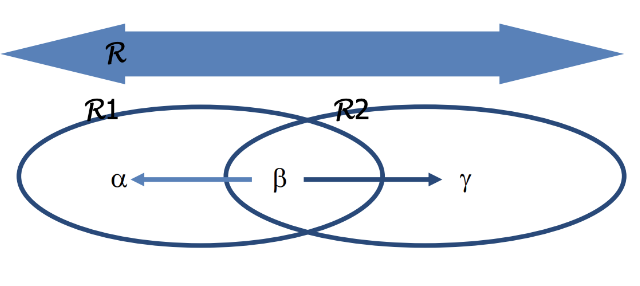
\includegraphics[width=.5\textwidth]{images/lossless_decomp.PNG}
\label{lossless_decomp}
\caption{Lossless Decompositon}
\end{figure}
Losslessness however, does not guarantee preservation of functional dependencies.

\section{Normal Form}
We want to formalize what is a good database design and formally model and enforce the properties we want in a good design. For this we need:
\begin{itemize}
\item A precise way to describe the property of the data - e.g. \textbf{functional dependency} as a precise way to describe \textbf{data redundancy}
\item Given the property of the data, describe the property of the DB design - \textbf{normal form}
\end{itemize}
What is a normal form. Database normalization is the process of structuring a relational database in accordance with a series of so-called normal forms in order to reduce data redundancy and improve data integrity. \\ Normal forms are common ways for normalization. For each normal form, we consider the following problems:
\begin{itemize}
\item Given a relation schema $R$, and a set of functional dependencies $FD$, how to decide whether $\{R, FD\}$ satisfies a given normal form.
\item Given $\{R, FD\}$ that satisfies a given normal form, what are the set of properties that it will have.
\item Given a relational schema $R$, and a set of functional dependencies $FD$, how to generate a new schema $R'$ such that $\{R', FD\}$ satisfies a given normal form.
\end{itemize}

\subsection{First Normal From (1NF)}
A database in first normal form contains only atomic domains. This means we do not allow non-atomic domains like arrays. This makes the concept of \textit{key} well defined (or, easier to define).

\subsection{Second Normal From (2NF)}
The second normal form tries to remove data redundancy. $\{R, FD\}$ is in second normal form if and only if every non-key attribute is minimally dependent on every key. Minimally dependent means that no attribute depends on part of the key. Relations that are not in second normal form experience the following problems:
\begin{itemize}
\item Insert Anomalies
\item Update Anomalies
\item Delete Anomalies
\end{itemize}
All of these can lead to redundant/inconsistent updates of the relations. In order to enforce the second normal form, we take the evil functional dependence and decompose the relation into multiple relations. This decomposition is lossless. The second normal form gets rid of insert anomalies but still experiences update and delete anomalies.

\subsection{Third Normal From (3NF)}
A relation $R$ is in third normal form if and only if for all functional dependencies $\alpha \to B$, at least one condition holds:
\begin{itemize}
\item $B \in \alpha$ ($\alpha \to B$ is a trivial FD)
\item $B$ is an attribute of at least one key
\item $\alpha$ is a superkey of $R$ (superkey = superset of some candidate keys)
\end{itemize}
Intuitively, if $\alpha \to B$ does not satisfy any of these conditions, $\alpha$ is a concept in its own right. The third normal form tries to get rid of \textit{transitive dependencies} (e.g. $A \to B ,B \to C)$. In 3NF, we still have update and delete anomalies.

\subsection{Boyce-Codd Normal Form}
A relation $R$ is in BCNF if and only if for all $\alpha \to B$, at least one condition holds:
\begin{itemize}
\item $B \in \alpha$ ($\alpha \to B$ is a trivial FD)
\item $\alpha$ is a superkey of $R$ (superkey = superset of some candidate keys)
\end{itemize}
Intuitively, in each relation, you only store the same information once.

\subsection{Decomposition Algorithm}
\begin{algorithm}
\caption{Decomposition($\mathcal{R}$)}
\begin{algorithmic}
\State $Result = \{\mathcal{R}\}$
\While{$\exists R_i$ in Result such that $R_i$ is not BCNF}
	\State Let $\alpha \to \beta$ be the evil FD
	\State $\mathcal{R}_i^1 = \alpha \cup \beta$
	\State $\mathcal{R}_i^2 = \mathcal{R}_i - \beta$
	\State $Result = (Result - \mathcal{R}_i) \cup \{\mathcal{R}_i^1, \mathcal{R}_i^2\}$
\EndWhile
\State \textbf{return} $Result$
\end{algorithmic}
\end{algorithm}
\newcommand{\R}{\mathcal{R}}
\noindent This algorithm takes as input a schema $\mathcal{R}$ and outputs a lossless decomposition $\mathcal{R}_1, ..., \R_n$ such that they will perfectly recover the information in $\R$ and $\R_1, ..., \R_n$ are in BCNF. BCNF does not preserve all functional dependencies, and it does not get rid of all data redundancies, only the ones that are caused by functional dependencies. 

\subsection{Synthesis Algorithm}
\begin{algorithm}
\caption{Synthesis($\R$)}
\begin{algorithmic}
\State Compute the minimal basis $F_c$ of $F$
\State For all $\alpha \to \beta \in F_c$, create $\R_{\alpha \cup \beta}(\alpha \cup \beta)$
\State If none of the above relations contains a superkey, add a relation with a key
\State Eliminate $\R_\alpha$ if there exists $\R_{\alpha'}$, such that $\alpha \subseteq \alpha'$
\end{algorithmic}
\end{algorithm}
\noindent This algorithm takes as input a schema $\R$ and outputs a lossless decomposition $\R_1, ..., \R_n$ that is in 3NF. The synthesis algorithm preserves all functional dependencies, but since it is not in BCNF it is not free of redundancies caused by functional dependencies.

\subsection{Multi-Value Dependency}
We formally define MVD as follows:
\begin{align*}
\alpha \to\to \beta \text{ for } R(\alpha, \beta, \gamma) \text{ iff.} \\
\forall t_1, t_2 \in R,\; t_1.\alpha = t2.\alpha \implies \exists t_3, t_4 \in R:\\
t_3.\alpha = t_4.\alpha = t_1.\alpha = t_2.\alpha; \\
t_3.\beta = t_1.\beta; t_4.\beta = t_2.\beta; \\
t_3.\gamma = t_2.\gamma; t_4.\gamma = t_1.\gamma;
\end{align*}
An intuitive way to think about MVD is to think about it in terms of joins. If we have $(\alpha \to\to \beta)$ we can decompose $R$ losslessly into $R_1 = \Pi_{\alpha, \beta}R$ and $R_2 = \Pi_{\alpha, \gamma}R$ such that $R = R_1 \Join R_2$.
The following laws hold for multi-value dependencies:
\begin{itemize}
\item \textbf{Trivial MVDs}\\
$\R(\alpha, \theta):\; \alpha \to\to \alpha\theta.\; (\alpha \to\to \R)$\\
Similarly: $\R(\alpha, \theta):\; \alpha \to\to \theta.\; (\alpha \to\to \R - \alpha)$\\
$\beta \subseteq \alpha \implies \alpha \to\to \beta$
\item \textbf{Promotion}\\
$\alpha \to \beta \implies \alpha \to\to \beta$\\
but $\alpha \to\to \beta \centernot\implies \alpha  \to \beta$
\item \textbf{Complement}\\
$\alpha \to\to\beta \implies \alpha \to\to \R - \alpha -\beta$
\item \textbf{Multi-Value Augmentation}\\
$\alpha \to\to \beta \land (\delta \subseteq \gamma) \implies \alpha\gamma \to\to \beta\delta$
\item \textbf{Multi-Value Transitivity}\\
$(\alpha \to\to \beta) \land (\beta \to\to \gamma) \implies \alpha \to\to \gamma$
\end{itemize}

\subsection{Fourth Normal Form}
A relation $R$ is in 4NF if and onlly if for all $\alpha \to\to\beta$, at least one condition holds:
\begin{itemize}
\item $\alpha \to\to \beta$ is trivial
\item $\alpha$ is a superkey of $R$ (superkey = supereset of some candidate keys)
\end{itemize}
The fourth normal form implies BCNF. 
\begin{algorithm}
\caption{Decompositon($\R$)}
\begin{algorithmic}
\State $Result = \{R\}$
\While{$\exists R_i$ in $Result$ such that $\R_i$ is not in 4NF}
	\State Let $\alpha \to\to \beta$ be the evil MVD
	\State $\R_i^1 = \alpha \cup \beta$
	\State $\R_i^2 = \R_i - \beta$
	\State $Result = (Result - \R_i) \cup \{\R_i^1, \R_i^2\}$
\EndWhile
\State \textbf{return} $Result$
\end{algorithmic}
\end{algorithm}
This algorithm takes a schema $\R$ and outputs a lossless decomposition $\R_1, ..., \R_2$ that is in 4NF.

\subsection{(De-)Normalization}
Now that we have seen all these normal forms the question of whether higher normalization is better poses itself. The answer is; it depends. There is always a tradeoff between performance and space. A denormalized database could be faster to read while redundancy incurs a higher overhead to maintain consistency.\\
What we have seen is that our normal forms provide:
\begin{itemize}
\item Lossless decomposition up to 4NF.
\item Preserving dependencies up to 3NF.
\end{itemize}
\begin{figure}[H]
\centering
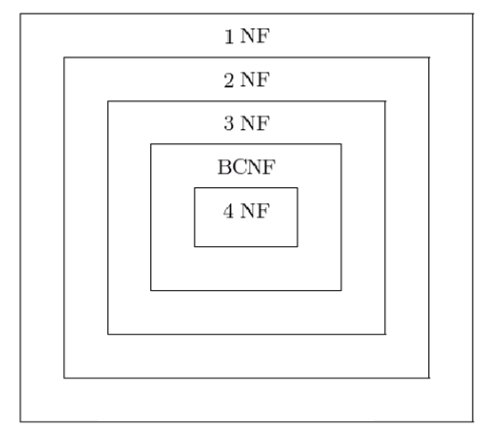
\includegraphics[width=.3\textwidth]{images/normal-forms.PNG}
\label{normal_forms}
\caption{Hierarchy of Normal Forms}
\end{figure}


\section{Database Systems}
In the real world, a database management system can be quite complex. In this course we focus on relational databases with disk-oriented architecture, where all data is stored on disk, the disk is larger and slower than memory and favors different access patterns.

\subsection{Overview}
A database management system can be abstracted into several layers, where an SQL query is passed in at the top, processed through the layers and the result is returned. The different layers try to hide complexity from layers above, they provide an interface to the upper layers and require services from the lower levels.
\begin{figure}[H]
\centering
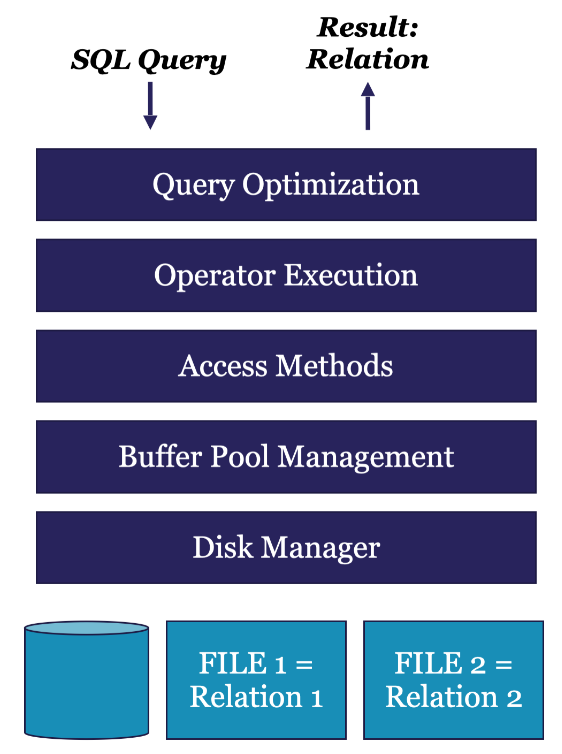
\includegraphics[width=.3\textwidth]{images/database_stack.PNG}
\label{database_stack}
\caption{Layers of a DBMS}
\end{figure}
\begin{itemize}
\item \textbf{Disk Manager}\\
The disk manager interacts with the disks, it allocates, deletes, and fetches pages. The idea is that no other layer has to interact with the disk directly.
\item \textbf{Buffer Pool Manager}\\
The buffer pool manager maintains an in-memory buffer such that all upper layers have the \textit{illusion} that the entire data is in memory and not on disk. It provides the functionality to fetch and update pages.
\item \textbf{Access Methods}\\
It provides different ways of accessing data from a relation such as \begin{itemize}
\item Sequential Scan
\item B-Tree Index
\item Hash Table
\item Sort
\end{itemize}
It provides a higher-level abstraction to access information in a table without interacting with the buffer or disk.
\item \textbf{Operator Execution}
This layer executes a relational algebra operator such as\begin{itemize}
\item Join
\item Projection
\item Select
\end{itemize}
It uses the access methods from the lower level to implement these operators.
\item \textbf{Query Optimization}\\
Given an SQL query, this layer generates a good execution plan (a tree of relational algebra operators). It uses the provided relational algebra operators from the lower level.
\end{itemize}

\subsection{Storage Hierarchy}
In an ideal world we would have private, infinitely large and fast, non-volatile and inexpensive memory. However, this is not the case. Our memory is structured like a pyramid. The faster and closer to the processor our memory is, the smaller, volatile and expensive it is. One access to main memory is already around 60 CPU cycles. A random access on a hard drive is closer to 10 million cycles. \\
Because our architecture is focused around hard drives, it is important to know how they work. A hard drive consists of multiple spinning disks and arms. On each arm there is a read/write head, which can read or write whatever part of the disk is currently beneath it. Only one head can read or write at any one point in time. The disk is split into multiple circular tracks. To read a specific track, the head is moved over the right track by an arm assembly. A block on the disk is a multiple of the fixed sector size. Now we take a look at a simplified performance model for hard drives:
\begin{figure}[H]
\begin{minipage}[t]{.5\textwidth}
\begin{itemize}
\item Seek / Rotate: $t_s, t_r$
\begin{itemize}
\item seek time (moving arms to position disk head on track)
\item rotational delay (waiting for block to rotate under head)
\end{itemize}
\item Transfer: $t_{tr}$
\begin{itemize}
\item transfer time (actually moving data to/from disk surface)
\end{itemize}
\item Random access $D$ times:
\begin{itemize}
\item $D(t_s + t_r + t_{tr})$
\end{itemize}
\item Sequential access $D$ times:
\begin{itemize}
\item $t_s + t_r + Dt_{tr}$
\end{itemize}
\end{itemize}
\end{minipage}
\begin{minipage}[t]{.5\textwidth}
\strut\vspace*{-\baselineskip}\newline
\centering
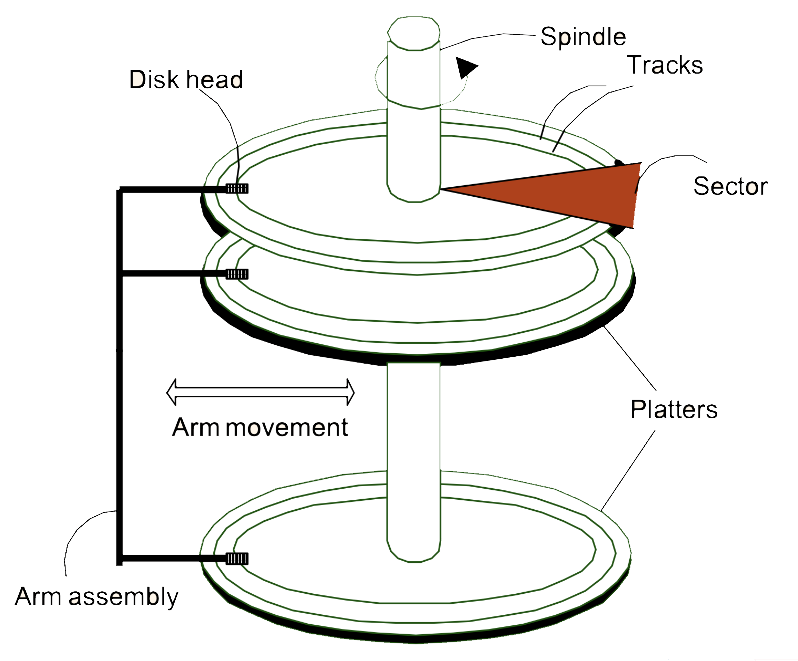
\includegraphics[width=\textwidth]{images/harddrive.PNG}
\label{harddrive}
\subcaption{Model of Hard Drive}
\end{minipage}
\end{figure}

In our model we focus on a simple hierarchy consisting of the hard drive, the DRAM and the CPU. Because the connection between DRAM and the CPU is dominatingly fast compared to the connection from hard drive to DRAM, we will focus on how to optimize data movement on the latter connection.

\subsection{Disk Manager}
The disk manager is the lowest layer of the DBMS software stack and it manages the space on disk. Higher levels call upon this layer to:\begin{itemize}
\item allocate/deallocate a page
\item read/write a page
\end{itemize}
A DBMS stores a database as one or more files on disk. Sqlite for example uses a single file. PostgreSQL on the other hand uses a collection of files. \\ The disk manager organizes the files as a collection of pages. A page is a fixed-size block of data that with a unique identifier. A page can contain tuples, meta-data, indexes or log records. A relation is stored as a collection of pages, where each page is a collection of tuples. There are multiple different ways to manage the collection of pages.

\subsubsection{Heap File}
A heap file is an unordered collection of pages, where tuples are stored in random order. Each record has a \textbf{Record ID} that consists of a Page ID and a Slot ID to identify in which page and where on the page the record is stored. There are two different ways to implement a heap file.\vspace{.3cm}\\
\textbf{Linked List}\\
A header page stores two pointers. One pointer points to the first entry in a linked list of free pages. The other pointer points to the first entry in a linked list of data pages. If a page is filled with tuples, it is moved from the free list to the data list.
\begin{figure}[H]
\centering
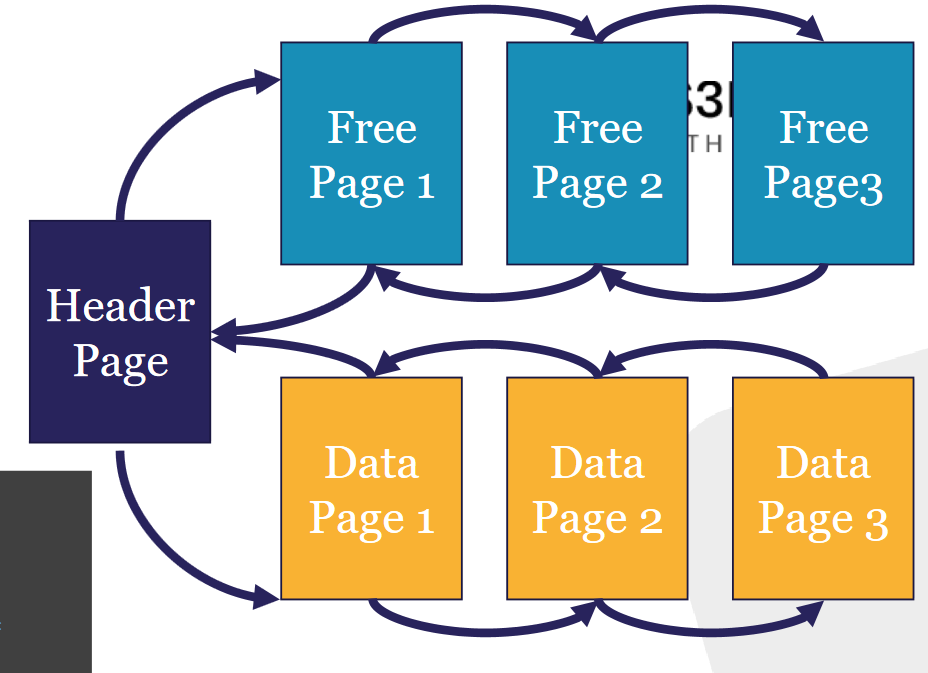
\includegraphics[width=.5\textwidth]{images/linked_list.PNG}
\label{linked_list}
\caption{Linked List Implementation}
\end{figure}
\textbf{Page Directory}\\
In a page directory, there is a set of header and data pages. A header page contains pointer to data pages as well as the number of free slots in those pages. The pages are allocated sequentially.
\begin{figure}[H]
\centering
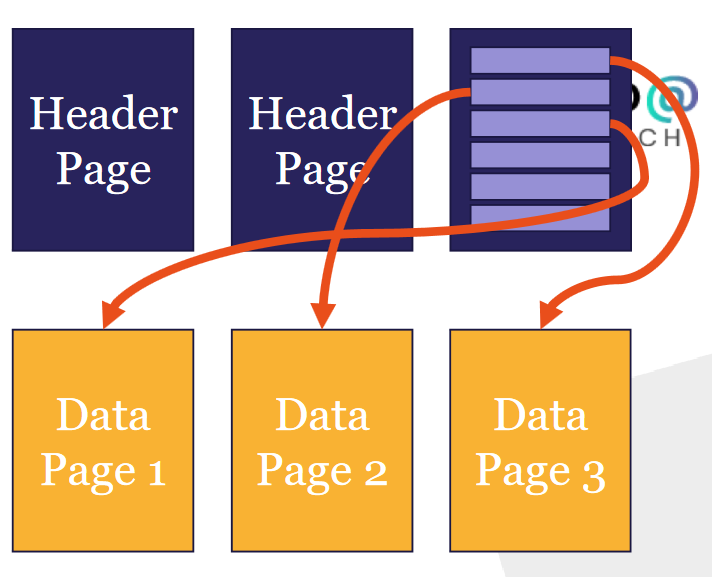
\includegraphics[width=.5\textwidth]{images/page_directory.PNG}
\label{page_directory}
\caption{Page Directory Implementation}
\end{figure}
\vspace{.2cm}
In the naive implementation using linked list, there will be free spaces on data pages here and there. There could also be free spaces when using page directory, but those spaces are easier to fill. \vspace{.3cm}\\
\textbf{Performance Model}\\
We assume the directory fits entirely into memory and is allocated. The number of pages we want to access is $D$.\vspace{.15cm}\\
\begin{tcolorbox}
\begin{minipage}[t]{.48\textwidth}
\textbf{Linked List}\\
Pages are randomly allocated on disk (worst case)
\begin{itemize}
\item Insert\\
$t_{s+r} + 2 \cdot t_{trans}$ (if page \#1 has slot available)
\item Find Record (by non-RID value)\\
$\frac{D}{2}(t_{s+r} + t_{trans}$ (In expectation)
\item Scan (all tuples)\\
$D(t_{s+r} + t_{trans})$
\end{itemize}
\end{minipage}
\begin{minipage}{.04\textwidth}
\hfill
\end{minipage}
\begin{minipage}[t]{.48\textwidth}
\textbf{Page Directory}\\
Pages are sequentially allocated on disk (best case)
\begin{itemize}
\item Insert\\
$t_{s+r} + 2 \cdot t_{trans}$ (if page \#1 has slot available)
\item Find Record (by non-RID value)\\
$(t_{s+r} + \frac{D}{2}t_{trans}$ (In expectation)
\item Scan (all tuples)\\
$t_{s+r} + D\cdot t_{trans}$
\end{itemize}
\end{minipage}
\end{tcolorbox}

\subsubsection{Page Layout}
Now we look at how data is stored inside a page. A page contains both a page header and actual data. The header contains meta-data like page size, DBMS version, compression/encryption information and checksum. In practice, often the header grows from the beginning of the page and the data from the end of the page. The data itself can be organized in different ways. \vspace{.2cm}\\
\textbf{Naive Strategy}\\
Each page contains fixed-length slots and in the header we keep track of the number of tuples in the page. With this implementation we run into trouble, when we encounter data that has a non-fixed length like strings. 
\begin{figure}[H]
\centering
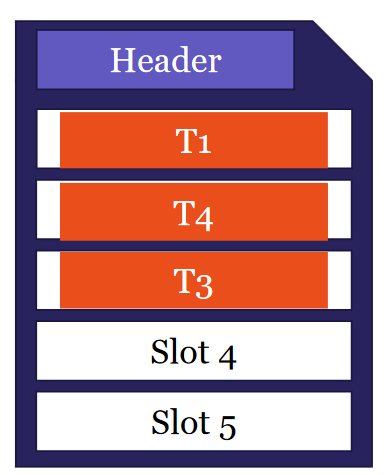
\includegraphics[width=.3\textwidth]{images/naive_strategy.PNG}
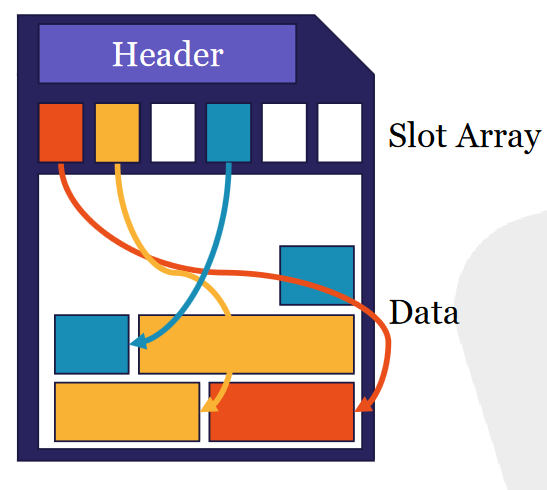
\includegraphics[width=.3\textwidth]{images/slotted_page.PNG}
\label{page_layout}
\caption{Implementation of Page Layout}
\end{figure}

\noindent\textbf{Slotted Page}\\
Another approach is to have slots of pointers. Each slot contains a pointer that then points to the start position of each data record. With this approach we can reorder the page without changing the Record ID.

\subsubsection{Tuple Layout}
\begin{itemize}
\item \textbf{Fixed Length Fields}
\begin{itemize}
\item direct access to these fields
\end{itemize}
\item \textbf{Variable Length Fields}
\begin{itemize}
\item store (length, pointer) as part of a fixed-length field
\item store payload information in a variable-length field
\item access in two steps: retrieve pointer + chase pointer
\end{itemize}
\item \textbf{NULL Values}
\begin{itemize}
\item Bitmap: set 1 if value of a field is NULL
\end{itemize}
\end{itemize}
Another option to store variable length field would be to separate the fields by special delimiter symbols.
\begin{figure}[H]
\centering
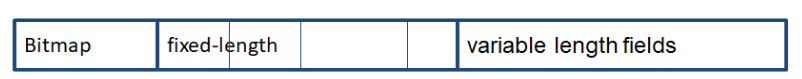
\includegraphics[width=.6\textwidth]{images/tuple_layout.PNG}
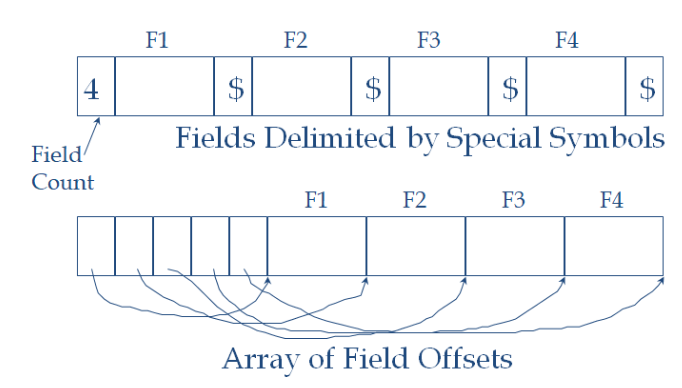
\includegraphics[width=.5\textwidth]{images/tuple_implementation.PNG}
\caption{Tuple Implementation}
\label{tuple_implementation}
\end{figure}

\subsubsection{Tuple Store vs Column Store}
For now we have looked at ways to store entire tuples together. However, we could also store the data in a column layout, depending on the workload we expect.
\begin{itemize}
\item \textbf{On-Line Transaction Processing}\\
Simple queries that read/update a small amount of data that is related to a single entity in the database.
\item \textbf{On-Line Analytical Processing}\\
Complex queries that read large portions of the database spanning multiple entities.
\end{itemize}
Our current layout always forces us to read the entire tuple even if we only need a few columns in a potentially huge table. This could waste a lot of I/O operations. One way of tackling this problem would be to store the values of the same column together.
\begin{itemize}
\item \textbf{Advantages}
\begin{itemize}
\item Reduces the amount of wasted I/O because the DBMS only read the data it needs
\item Easier data compression, since we only have to store each value that appears in the column once.
\end{itemize}
\item \textbf{Disadvantages}
\begin{itemize}
\item Slow for point queries, inserts, updates and deletes since we need to search to tuple attributes one-by-one.
\end{itemize}
\end{itemize}

\subsection{Buffer Manager}
\begin{wrapfigure}{r}{.5\textwidth}
\centering
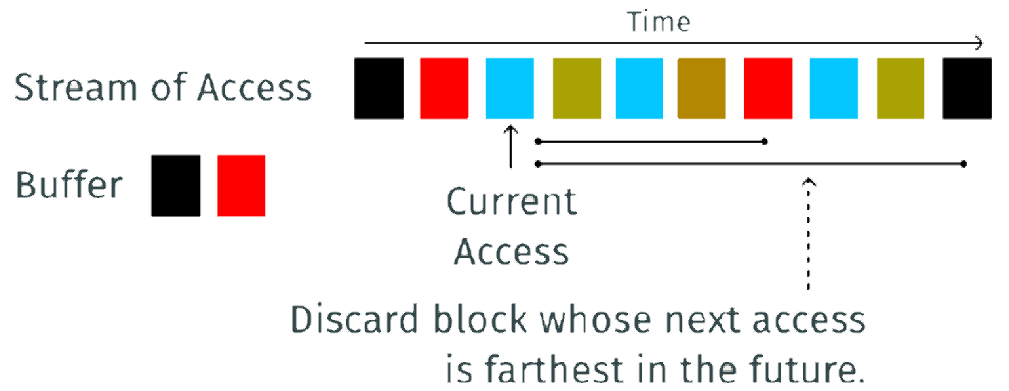
\includegraphics[width=.5\textwidth]{images/belady.PNG}
\label{belady}
\caption{Optimal Strategy}
\end{wrapfigure}
The buffer manager acts like the intermediate layer between the system and disk manager. It tries to provide the illusion that all the data is in DRAM. The core question of the buffer manager is how to optimally replace pages in the buffer. The optimal strategy depends on whether we know what is going to happen in the future.
\vspace{.2cm}\\
If we know the future access pattern, we discard the block whose next access is the farthest in the future. This strategy is proven to be optimal and called \textbf{Bélády's Min}. \vspace{.2cm}\\
But how do we chose which page to evict in practice, where we do not always know the future. One way to do it is called \textbf{Least Recently Used}. For each page in the buffer pool, we keep track of the time it was last used. We then always evict the page, that has been used the furthest in the past. This method works well for repeated accesses to popular pages. We encounter a problem when the number of pages exceeds the number of buffer slots. If we then sequentially access all the data, we are going to miss on every request. This is called \textbf{sequential flooding}. But we know that LRU is at most twice as bad as the optimal strategy when given twice the memory. \vspace{.2cm}\\
Another common strategy is called \textbf{Most Recently Used}. For each page in the buffer pool, we keep track of the time it was last used. We then always evict the page that hast been used the most recently.\vspace{.2cm}\\
How well a replacement strategy performs depends on the access pattern. Such access patterns could be
\begin{itemize}
\item Sequential: Table Scans
\item Hierarchical: Index Scans
\item Random: Index Lookup
\item Cyclic: Nested Loop
\end{itemize}
Different replacement strategies work better for different cases. In many cases, the DBMS knows the pattern and can tell the buffer manager.

\subsection{Access Methods}
This layer provides different ways of accessing data from a relation. To the upper layer it provides an abstraction to access information in a table without interacting with the buffer or disk. It conducts a sequence of invocations to the buffer manager to access information in a relation. There are different ways to conduct the accesses.

\subsubsection{Sequential Scan}
In the sequential scan we tell the buffer manager to sequentially bring all the pages of the relation and scan the tuples. It would look something like
\begin{itemize}
\item Bring me page 1, scan all the tuples and check
\item Bring me page 2, scan all the tuples and check
\item Bring me page 3, scan all the tuples and check
\end{itemize}
The cost of a sequential scan to read $D$ pages:
\begin{itemize}
\item When pages are sequentially allocated\\
$t_{s+r} + D(t_{trans}$
\item WHen pages are randomly allocated\\
$D(t_{s+r} + t_{trans})$
\end{itemize}
If we also update and write back the tuples, we need one more $t_{trans}$.

\subsubsection{Index}
To index a relation is to build a data structure $f$ over the relation $R$. That given information about a tuple, we can find the Record ID.
\begin{align*}
f("Age = 5") \mapsto RID
\end{align*}
Usually, evaluating $f$ is cheaper than a sequential scan of the whole relation. There are different kinds of indexes such as B-Tree, Hash table, Learned index and many more.

\subsubsection{B-Tree (B+ Tree)}
A B-Tree is a self-balancing tree data structure that keeps data sorted. As usual in balanced trees we have $\bigo (\log n)$ asymptotic complexity for search, insertion and deletion. It is a generalization of a binary search tree in which each node contains more than two children. It is optimized for system that read and write large blocks of data (i.e. read in pages).\\
A B-Tree is a $M$-way search tree that is:
\begin{itemize}
\item Perfectly balanced
\item Every inner node other than the root, is at least half-full
\item Every inner node with $k$ keys has $k+1$ non-null children.
\end{itemize}
Each inner node's keys act as separation values which divide its subtrees. For example if an inner node has 3 child nodes then it must have 2 keys: $a_1$ and $a_2$. All values in the leftmost subtree will be less than $a_1$, all values in the middle subtree will be between $a_1$ and $a_2$, and all values in the rightmost subtree will be greater than $a_2$.\\
There are two different flavors of B-Trees. In a \textbf{clustered} B-Tree, the leaf nodes contain the actual tuple. It is only possible to have one such clustered B-Tree per relation. In an \textbf{unclustered} B-Tree, the leaf node contains the Record Id, pointing to the tuple.
\begin{figure}[H]
\centering
\includegraphics[width=.5\textwidth]{images/btree.PNG}
\label{btree}
\caption{B-Tree}
\end{figure}
We assume a B-Tree with node size $M$ and the total number of tuples $N$. The depth of the B-Tree is $\log_M N$. To find a single key:
\begin{itemize}
\item \#I/O, Unclustered B-Tree:
\begin{itemize}
\item $\log_M N + 1$
\item $\log_M N$: Read one pager per level
\item $1$: Read the actual tuple
\end{itemize}
\item \#I/O, Clustered B-Tree:
\begin{itemize}
\item $\log_M N$
\end{itemize}
\end{itemize}
If we want to find all the tuples in a range of keys:
\begin{itemize}
\item \#I/O, Unclusterd B-Tree:
\begin{itemize}
\item $\log_M N + \frac{\#tuples}{tuple\_per\_page} + \#tuples$ (worst case)
\item $\log_M N$: REad one page per level
\item $\frac{\#tuples}{tuple\_per\_page}$: \#leaf pages one need to read to get all RIDs
\item $\#tuples$: Cost of reading all tuples unclustered, which is one I/O operation per result in the worst case.
\end{itemize}
\item \#I/O, Clustered B-Tree
\begin{itemize}
\item $\log_M N + \frac{\#tuples}{tuple\_per\_page}$
\item $tuple\_per\_page$ is lower, since in a clustered B-Tree the entire tuple is stored.
\end{itemize}
\end{itemize}
To insert a tuple into a B-Tree, we find the right leaf node $L$ and insert our tuple. If $L$ has enough space we are done, otherwise we split $L$ and insert the key into the parent of $L$. Splitting is done by finding the median key.\\
To delete a tuple, we find the right leaf node $L$ and remove the entry. If $L$ is at least half full we are done, otherwise we might have to merge two leaf nodes or borrow a tuple from a neighbor and update the parents.\vspace{.2cm}\\
To create a B-Tree in PostgreSQL we can use the following command:
\begin{lstlisting}[language=SQL]
CREATE INDEX name ON table USING btree (column);
\end{lstlisting}
Since B-Tree is the default index we can also omit the \textit{USING} clause.

\subsubsection{Hash Table}
Hash tables are a different kind of index where we try to achieve constant access time for point queries. What we hope for in hash functions is that the probability of collision is very small. Still because the probability is non-zero we have to deal with potential collisions. The way hash tables work is that we feed the tuple (or parts of it) into the hash function which then returns the index of a slot. There are different ways to approach collision handling:
\begin{itemize}
\item \textbf{Closed Hashing}\\
In closed hashing we know how many elements we are trying to hash. This means that each slot stores the tuple itself or at most a single Record ID. A way to deal with collisions is the \textbf{Linear Probe}, where we first try to insert the element at the slot given by the hash function. If this slot is already occupied, we sequentially go to the next slot until we find a free one. This creates some issues when deleting entries as we have to maintain all the sequential hops with special values. Linear Probe is very cache-efficient but also very sensitive to the chosen hash function. Given that the hash function is reasonably good, this method performs adequately well. There are also other methods to deal with collisions in closed hashing:
\begin{itemize}
\item Double Hashing - Offset the search of a free slot by a second hash value
\item Quadratic Probing - Offset the search of a free slot by $1^2, 2^2, 3^2, ...$
\end{itemize}
\item \textbf{Open Hashing}\\
In open hashing we do not know how many elements we are dealing with. Potentially even more than our hash table has slots. So instead of a single Record ID, we store a linked list of tuples or Record IDs. This technique is called \textbf{chained hashing}. If a tuple falls into an already occupied slot, the tuple is appended to the linked list. To retrieve a value, we have to search the given linked list.
\end{itemize}

\subsection{Operator Execution}
This layer executes relational algebra operators. It uses the different access methods from the layer below to implement these operators. To the upper layer it provides the ability to execute those operators.

\subsubsection{Select}
To implement the select operator $\sigma_C(R)$ for a predicate $C$ we have two different methods. 
\begin{addmargin}{-.5cm}
\begin{itemize}
\item \textbf{Sequential Scan over Heap File}\\
We bring the pages of the heap file into DRAM one-by-one. For each page, we scan all of its tuples and check for the predicate $C$. If the predicate evaluates to true, we output the tuple.\\
To evaluate the I/O cost we assume that the relation $R$ has $|R|$ tuples on $B(R)$ pages. The buffer size of the system is $M$ pages. The cost to read all pages is $B(R)$. The cost to write the tuples is $\alpha(C, R)\cdot B(R)$, where $\alpha(C, R)$ is a key constant called \textbf{selectivity}, which is the relative number of tuples in $R$ that satisfy the condition $C$ divided.\\
The total cost of a sequential scan is: $B(R) + \alpha(C, R) \cdot B(R)$.
\item \textbf{Index Scan}\\
When the predicate $C$ is a check for equivalence or greater/less we can use the B-Tree index to check the condition.\\
In an unclustered B-Tree we search for the right leaf node, scan the index and then fetch the corresponding tuple in the heap file.\\
In a clustered B-Tree we search for the right leaf node and return the tuples along the way.\\
To evaluate the I/O cost we assume the same metrics as above.
\begin{tcolorbox}
\begin{minipage}[t]{.48\textwidth}
For unclustered B-Tree:\\
The cost to find the leaf is $\bigo(\log |R|)$. The cost fetch the tuples is $\bigo (\alpha(C, R) \cdot |R|)$ and to write $\alpha(C, R)\cdot B(R)$.\\
The total cost is $\bigo(\log |R| + \alpha(C, R) \cdot |R| + \alpha(C, R)\cdot B(R))$.
\end{minipage}
\begin{minipage}[t]{.04\textwidth}
\hfill
\end{minipage}
\begin{minipage}[t]{.48\textwidth}
For clustered B-Tree:\\
The cost to find the leaf is $\bigo(\log |R|)$. The cost to fetch the tuples is $\bigo (\alpha(C, R) \cdot B(R))$ and to write $\alpha(C,R)\cdot B(R)$.\\
The total cost is $\bigo (\log |R| + 2\cdot \alpha(C, R) \cdot B(R))$.
\end{minipage}
\end{tcolorbox}
\end{itemize}
\end{addmargin}
Whether we should use sequential scan or index scan depends on a lot of factors such as the relative speed of sequential to random access as well as the selectivity and whether the index is clustered or not. To factor this in and make an estimate on which mode is the fastest is the job of the DBMS.

\subsubsection{Sort}
To implement the select operator that sorts a relation $R$ on an attribute $A$ we have several options again. If we have a clustered B-Tree on $A$ is is very straight forward. We simply scan the B-Tree leaf nodes and return the trivially sorted result.\\
If we have an unclustered B-Tree on $A$ the job is equally simple but a lot slower. Since we still index the tuples in an ordered fashion we only have to read the tuple references in order. However, since the B-Tree is unclustered and for each tuple we have to chase a reference we have one random access per tuple in the worst case.\vspace{.3cm}\\
\textbf{Sorting Tuples on Disk}\\
In case we do not have a B-Tree index or want to sort the actual data on disk we might think about QuickSort. However, QuickSort is not designed to be I/O efficient and therefore doesn't have very good locality. Since we are dealing with block story, we need to worry more about locality. Whenever we read a page, we better take advantage of every tuple in that page.\\
This can be done with the \textbf{external sort} algorithm.\\
We assume to have $N$ pages on disk to sort and a $B$-page buffer in memory. In the case that $N < B$, we simply load all the data into the buffer and sort it using QuickSort. In the more interesting case where $N > B$ we apply an algorithm that is similar to MergeSort.
\begin{itemize}
\item Sort each page individually
\item Combine pages
\end{itemize}
The single pages can easily be sorted with QuickSort. With a 3-page buffer we can sort 2 sorted files. We simultaneously load the first elements of both files into the buffer, choose the smaller one between the too and output it to the third buffer. Then we take the next element from the file we chose the first tuple and repeat the process until both files are merged together.\\
The total cost of sorting is $\bigo (( \log_{B-1} (\frac{N}{B}) + 1) N )$.

\subsubsection{Join}
\begin{itemize}
\item \textbf{Nested Loop Join}\\
\begin{algorithm}[h]
\caption{Nested Loop Join ($R \Join_\theta S$)}
\begin{algorithmic}
\For{each tuple $r$ in $R$}
	\For{each tuple $s$ in $S$}
		\If{$\theta(r, s)$}
			\State append $(r, s)$ to result
		\EndIf
	\EndFor
\EndFor
\end{algorithmic}
\end{algorithm}
This is the most naive way to perform a join operation. We simply iterate through each tuple combination with two for-Loops and check the condition. The cost of this operation depends on the join order and buffer size. For a buffer size of 3 the cost, disregarding the operations to write the result out is $B(R) + |R| \cdot B(S)$. Usually we want the smaller relation to be in the outer loop, however, if we have a large buffer $(M \geq B(S) + 2$ we can cache the smaller relation and want it in the inner loop.
\item \textbf{Block Nested Loop Join}\\
This version of the nested loop join performs loop unrolling to partition the relations into blocks and iterate over those instead of the entire relations. This increases locality and therefore performance by reducing I/O operations by up to 2 orders of magnitude.
\begin{algorithm}[h]
\caption{Block Nested Loop Join($R \Join_\theta S$)}
\begin{algorithmic}
\For{each block $BR$ in $R$}
	\For{each block $BS$ in $S$}
		\For{each tuple $r$ in $BR$}
			\For{each tuple $s$ in $S$}
				\If{$\theta(r, s)$}
					\State append $(r, s)$ to result
				\EndIf
			\EndFor
		\EndFor
	\EndFor
\EndFor
\end{algorithmic}
\end{algorithm}
The cost of a join using blocked loops is with a buffer size of 3 is $B(R) + B(R) \cdot B)S)$. If we have a larger buffer of $M > 3$ we can partition $S$ into $B(s) / (M-2)$ chunks which reduces our cost to $B(S) + B(R)\cdot (B(S) / (M-2))$. 
\item \textbf{Index Nested Loop Join}\\
This version leverages the search index on a relation $S$.
\begin{algorithm}[H]
\caption{Index Nested Loop Join}
\begin{algorithmic}
\For{each tuple $r$ in $R$}
	\For{each tuple $s$ in $IndexScan(S, r, \theta)$}
		\State append $(r, s)$ to result
	\EndFor
\EndFor
\end{algorithmic}
\end{algorithm} 
The cost model of this is very simple, it is $B(R) + |R| \cdot C$, where $C$ is the cost of a lookup in the index. This can be very efficient. Because you usually have the first few levels of a B-Tree in the buffer, you can retrieve a lot of tuples with very few I/O operations. 
However, this kind of join is restricted to operations like $=, >, <$.
\item \textbf{Sort Merge Join}\\
To conduct equivalence joins or joins with $<, >$ we can first sort both relations. Once we have sorted both relations we compare them similarly to external sort. We load the first page from both relations into the buffer, since both relations are sorted it is easy to find matches and discard tuples without matches.\\
The cost of a sort merge join is $B(R) + B(S) + Sort(R) + Sort(S)$.

\item \textbf{Hash Join}\\
There is an even faster way to conduct equivalence joins using hash tables.
\begin{algorithm}[H]
\caption{Hash Join $R \Join_\theta S)$}
\begin{algorithmic}
\State build hash table $HT$ for $R$
\For{each tuple $s$ in $S$}
	\If{$h(s)$ in $HT$}
		\State append tuples $(r, s)$ where $\theta(r, s)$ to result
	\EndIf
\EndFor
\end{algorithmic}
\end{algorithm}
This algorithm is incredibly efficient and only passes both relations once, if the hash table fits into memory that is. The cost is $B(R) + B(S)$.
\item \textbf{Grace Hash Join}\\
If the hash tale does not fit into memory completely we can perform a grace hash join. We also create a hash table for $R$, that sadly is too large for the memory. Therefore, we partition the hash table $HT$ as well as the relation $S$ into 3 (or $n$) partitions using another hash function. With these partitions we then can perform the hash join. The cost of this is $3(B(R) + B(S))$ (or $n$ when doing more partitions).
\begin{figure}[H]
\centering
\includegraphics[width=.6\textwidth]{images/grace_join.PNG}
\label{grace_join}
\caption{Grace Hash Join}
\end{figure}
\end{itemize}
As an overview again the different types of joins and on which predicates they can join.
\begin{tcolorbox}
\begin{minipage}[t]{.4\textwidth}
\textbf{Join Type}
\begin{itemize}
\item Nested Loop Join
\item Block Nested Loop Join
\item Index Nested Loop Join
\item Sort Merge Join
\item Hash Join
\end{itemize}
\end{minipage}
\begin{minipage}[t]{.6\textwidth}
\textbf{Join Predicates}
\begin{itemize}
\item $\theta(r, s)$
\item $\theta(r, s)$
\item B-Tree: $r.a = s.b,\; r.a < s.b,\; r.a > s.b;$ Hash Index: $r.a = s.b$
\item $r.a = s.b,\; r.a < s.b,\;r.a > s.b$
\item $r.a = s.b$
\end{itemize}
\end{minipage}
\end{tcolorbox}

\subsection{Query Optimization}
The query optimization layer should, given an SQL query, generate a good execution plan (a tree of realtional algebra ooperatiors). The fundamental questions of this layer are; How to run a physical plan, given that we know how to run each operator? How to search for the best physical plan?

\subsubsection{Execution Model}
The execution model is the way in which we put the operators together.\vspace{.3cm}\\
\textbf{Iterator Model}\\
In the iterator model, each operator is an iterator - it takes as input a set of streams of tuples and outputs a stream of tuples. A stream provides a \textit{next()} interface. In this model the query plan is a tree of iterators. To get the result, we call $root.next()$ over and over again. This model mimics a data flow from the bottom to the top.
\begin{figure}[H]
\centering
\includegraphics[width=.5\textwidth]{images/iterator.PNG}
\label{iterator}
\caption{Iterator Model}
\end{figure}
This model is a very generic interface that hides the information very well and is easy to implement. There are is no overhead in terms of main memory and it supports pipelining, parallelism and distribution. However, it produces a high overhead of method calls and has poor instruction cache locality.\vspace{.3cm}\\
\textbf{Materialization Model}\\
In the materialization model, each operator processes its input all at once and emits its output all at once. This model is good when the intermediate results are not too much larger than the final result. OLTP is a good example workload while OLAP might not be best suited for this model.
\begin{figure}[H]
\centering
\includegraphics[width=.5\textwidth]{images/materialization.PNG}
\label{materialization}
\caption{Materialization Model}
\end{figure}
\textbf{Vectorization Model}\\
The vectorization model operates similarly to the iterator model, but instead of returning a single tuple on invocation, the operator returns a batch of tuples. This greatly reduces the number of invocations per operator and allows for operators to use vectorized (SIMD, AVX) instructions to process batches of tuples, which makes this mode good for OLAP workloads.

\subsubsection{Search Space}
Given a logical plan as input, there are different ways that one can construct a physical plan. For example we could change the join order or execute selection at different times. We now define a set of transformations called \textbf{query rewriting rules} that will take as input a query plan and output an equivalent query plan.
\begin{itemize}
\item $\sigma_{\theta_1 \land \theta_2}(E) = \sigma_{\theta_1}(\sigma_{\theta_2} (E))$\\
Conjunctive selection operations can be deconstructed into a sequence of individual selections.
\item $\sigma_{\theta_1}(\sigma_{\theta_2}(E)) = \sigma_{\theta_2}(\sigma_{\theta_1}(E))$\\
Selection operations are commutative.
\item $\Pi_{t_1}(\Pi_{t_2}(E)) = \Pi_{t_1}(E)$\\
Only the last in a sequence of projection operations is needed, the others can be omitted.
\item $\sigma_\theta(E_1 \times E_2) = E_1 \Join_\theta E_2$\\
$\sigma_{\theta_1}(E_1 \Join_{\theta_2} E_2) = E_1 \Join_{\theta_1 \land \theta_2} E_2$\\
Selections can be combined with Cartesian products and theta joins.
\item $E_1 \Join_\theta E_2 = E_2 \Join_\theta E_1$\\
Theta-join operations (and natural joins) are commutative.
\item $(E_1 \Join E_2) \Join E_3 = E_1 \Join (E_2 \Join E_3)$\\
Natural join operations are associative.
\item $\sigma_\theta (E_1 \Join E_2) = \sigma_\theta(E_1) \Join (E_2)$\\
Selection can be pushed down, if $\theta$ only involves attributes in $E_1$.
\item $\Pi_{L_1 \cup L_2}(E_1 \Join_\theta E_2) = (\Pi_{L_1}(E_1)) \Join_\theta (\Pi_{L_2}(E_2))$\\
The projection operation distributes over the theta join operation if $\theta$ only involves attributes from $L_1 \cup L_2$.
\item $E_1 \cup E_2 = E_2 \cup E_1, \; E_1 \cap E_2 = E_2 \cap E_1$\\
$(E_1 \cup E_2) \cup E_3 = E_1 \cup (E_2 \cup E_3), \; (E_1 \cap E_2) \cap E_3 = E_1 \cap (E_2 \cap E_3)$\\
The set operations union and intersection are commutative and associative.
\item $\sigma_\theta(E_1 - E_2) = \sigma_\theta(E_1) - \sigma_\theta(E_2)$\\
$\sigma_\theta(E_1 \cup E_2) = \sigma_\theta(E_1) \cup \sigma_\theta(E_2)$\\
$\sigma_\theta(E_1 \cap E_2) = \sigma_\theta(E_1) \cap \sigma_\theta(E_2)$\\
The selection operator distributes over $\cup, \cap$, and $-$.
\item $\Pi_L(E_1 \cup E_2) = (\Pi_L(E_1)) \cup (\Pi_L(E_2))$\\
The projection operation distributes over union.
\end{itemize}
All these rules give us a way to generate physical plans.

\subsubsection{Cost Model}
The cost model provides a way to estimate the performance of a given physical query plan without actually running the query. We have already seen cost estimation for each operator. While some constants like number of pages or number of tuples are query-independent, other factors like selectivity are query-dependent. The core concept is \textbf{cardinality estimation}. We need to figure out how many tuples a query would return.\\
One way to estimate the number of tuples is by creating histograms over attribute. The cost is ammortized since we can use the histogram over many queries. However, this only works if the values are distinct. For continuous values the histogram needs to use bins. Another difficulty in estimation is in correlated queries. There the attributes are assumed to be independent which can give inaccurate answers. Another option is to build multi-dimensional histograms, but this is very expensive.

\subsubsection{Search Algorithm}
Now that we are able to generate semantically equivalent plans, the first idea is to enumerate all possible executions and choose the cheapest one. However, since queries can be reasonably complex, the search space is incredibly huge. There are already $4^n$ ways to join $n$ relations.\\
A first approach could be to constrain the search space, i.e. limit the possible execution plans we look at. One way is to only consider left-deep join trees, because left-deep trees allow to generate fully pipelined plans where intermediate results don't have to be written to temporary files. The best plan in the limited search space can then be decided by dynamic programming but it is still very slow.\\
Another approach could be heuristic-based. Since cost-based optimization is very expensive, systems may use heuristics to reduce the number of choices that must be made in a cost-base fashion. Common heuristics are:
\begin{itemize}
\item Perform selection early (reduces the number of tuples)
\item Perform projection early (reduces the number of attributes)
\item Perform most restrictive selection and join operations before similar operations
\end{itemize}

\section{Transactions \& ACID}
What motivates the notion of transactions are concurrent database accesses and resilience to system failures. If we imagine a DBMS with a single thread that has to process two queries at the same time. The system could interleave the two executions which can lead to a variety of inconsistencies. Inconsistencies can be experienced on attribute-, tuple- or table-level or occur from multiple statements.
One way to interleave the instructions is called a \textbf{schedule}.\\
The second motivation is the dealing with system failure. When the system fails during changes to the database, there are three possible states:
\begin{itemize}
\item None of the changes are in
\item All of the changes are in
\item Some of the changes are in
\end{itemize}
In database systems we want to avoid the last state. The way to avoid this are transactions. A transaction is a sequence of one or more SQL operations treated as a unit. Concurrent transactions appear to run in isolation (i.e. sequentially). If the system fails, each transaction's changes are reflected either entirely or not at all. A transaction is initiated with the keyword \textit{BEGIN} and terminated with the keyword \textit{COMMIT} or \textit{ABORT}. If the transaction commits, the changes of the transaction have been made persistent. If the transaction aborts, the database rollbacks and changes are undone.\\
\begin{minipage}{.48\textwidth}
\begin{lstlisting}[language=SQL]
BEGIN;
SQL
SQL
COMMIT;
\end{lstlisting}
\end{minipage}
\begin{minipage}{.04\textwidth}
\hfill
\end{minipage}
\begin{minipage}{.48\textwidth}
\begin{lstlisting}[language=SQL]
BEGIN;
SQL
SQL
ABORT;
\end{lstlisting}
\end{minipage}

\subsection{ACID}
ACID stands for the desired properties of transactions
\begin{enumerate}
\item[\textbf{A}] Atomicity - a transaction is executed in its entirety or not at all
\item[\textbf{C}] Consistency - a transaction executed in its entirety over a consistent DB produces a consistent DB
\item[\textbf{I}] Isolation - a transaction executes as if it were alone in the system
\item[\textbf{D}] Durability - committed changes of a transaction are never lost - can be recovered
\end{enumerate}
A naive way to implement transactions would be to execute the transactions one-by-one. Before \textit{BEGIN}, we dump the whole database to a new file and before \textit{COMMIT} we overwrite the original file. However, this is extremely slow and incurs huge overhead to copy the whole database every time. Luckily, this is not how current database systems work.


\subsection{Atomicity}
Atomicity requires transactions to be all-or-nothing, no transaction is left half done. The effects are either all in the database or not in the database at all. 
\subsection{Consistency}
Consistency requires transactions to keep consistent states. Given all integrity constraints hold when the transaction begins, all constraints must hold when the transaction ends. During the transaction some constraints may be violated. However, serializability (isolation) implies that constraints always hold, if each transaction is correct.
\subsection{Isolation}
Isolation allows execution to be interleaved but the execution must be \textbf{equivalent to some sequential order} of all transactions. An execution that is equivalent to a serial execution is called \textbf{serializable}. It is possible that different serial executions lead to different results but that is acceptable from the DBMS perspective. If we need one possibility over another, this should be enforced by the application and not the DBMS.\\
Achieving isolation as defined above might be expensive and in some cases a weaker notion of isolation would suffice. Therefore, databases provide different isolation levels. Isolation levels are a property of each individual transaction. The isolation levels are defined by anomalous behaviors that are allowed in each level.
\begin{figure}[H]
\centering
\includegraphics[width=.3\textwidth]{images/isolation_levels.PNG}
\label{isolation_levels}
\caption{Isolation Levels}
\end{figure}

\subsubsection{Read Uncommitted}
The \textit{read uncommitted} level allows a transaction to perform dirty reads. A read is dirty if it was written by a different uncommitted transaction. The dirty read might be a value that never exists in the database when the other transaction aborts. \\e 

\subsubsection{Read Committed}
The \textit{read committed} level does not allow dirty reads, it is stronger than \textit{read uncommitted} but still doesn't guarantee serializability. Another transaction could update and commit in the meantime and change values. The execution is therefore, not equal to any sequential execution.
\begin{figure}[H]
\centering
\includegraphics[width=.3\textwidth]{images/read_committed.PNG}
\label{read_committed}
\caption{Read Committed but not Serializable}
\end{figure}

\subsubsection{Repeatable Read}
The \textit{repeatable read} level does not allow dirty reads and additionally, an item read multiple times cannot change value. This notion is stronger than \textit{read committed} but still does not guarantee serializability. Another transaction could insert new tuples or change different attributes such. 
\begin{figure}[H]
\centering
\includegraphics[width=.3\textwidth]{images/repeatable_read.PNG}
\label{repeatable_read.PNG}
\caption{Repeatable Read but not Serializable}
\end{figure}

\subsection{Durability}
Durability requires changes of transactions to be persistent in the database. If the system crashes after a transaction committed, all effects must remain in the database.

\subsection{Formal Definition}
A database is a fixed set of named data objects (e.g. A, B, C...). In practice, transactions can create new objects but here we assume that they cannot do that. A transaction is a sequence of read and write operations:
\begin{itemize}
\item $a \gets R(A)$: read object $A$ into variable $a$
\item $W(B, b)$: write the value of variable $b$ into object $b$\\
We assume that the moment we write, the changes are reflected in the database.
\end{itemize}
A new transaction starts with \textit{BEGIN} and stops with either \textit{COMMIT} or \textit{ABORT}. If the transaction commits, all changes are saved. If the transaction aborts, all changes are undone so ti is like the transaction never happened.

\subsection{Conflict Serializability}
The serializability of a schedule is not decided by solely it's I/O pattern. \textbf{Conflict serializability} is a stronger notion of serializability that only depends on the I/O pattern and is thus easier to handle for the DBMS. \\
We call a schedule conflict serializable if the schedule is conflict equivalent to some serial schedule. Two schedules are conflict equivalent if and only if
\begin{itemize}
\item They involve the same actions of the same transactions
\item Every pair of conflicting actions is ordered in the same way
\end{itemize}
There are different types of actions that conflict:
\begin{itemize}
\item Trivial Conflicts - two different operations from the same transaction are always conflicting, i.e. we cannot reorder within transactions
\item Read-Write Conflict - leads to unrepeatable reads
\item Write-Read Conflict - leads to dirty reads
\item Write-Write Conflict - leads to overwriting uncommitted data
\end{itemize}
\begin{figure}[H]
\centering
\includegraphics[width=.45\textwidth]{images/read-write.PNG}
\includegraphics[width=.45\textwidth]{images/read-read.PNG}
\includegraphics[width=.45\textwidth]{images/write-write.PNG}
\label{conflicts}
\caption{Different Types of Conflicts}
\end{figure}
Conflict serializable schedules are a subset of serializable schedules and it is enforced by most DBMS.

\subsubsection{Decide Conflict Serializability}
A naive way to check if a schedule is conflict serializable is to go from the definition and perform the swaps, however, there is a better way. We can construct a dependency graph where
\begin{itemize}
\item Each transaction is a Node in the graph.
\item There is an edge from $T_i$ to $T_j$ if an operator $o_i$ in $T_i$ is in conflict with an operation $o_j$ in $T_j$ and $o_j$ appears earlier than $o_j$.
\end{itemize}
A schedule is conflict serializable if and only if its dependency graph is acyclic.

\subsection{Locking}
A pessimistic approach to enforcing isolation is to proactively prevent non-serializable schedules from happening via locking. The idea is that before the system accesses the data object $X$, it locks $X$ such that other transactions cannot access it at the same time and the system only releases the lock when it is safe to do so.\\
There are also different types of locks. For example, we could have shared and exclusive locks that are required for read and write operations respectively. Intuitively, multiple read operations can happen at the same time while writing needs exclusivity.
\begin{figure}[H]
\centering
\includegraphics[width=.5\textwidth]{images/lock_types.PNG}
\label{lock_types}
\caption{Lock Types}
\end{figure}
It is important to realize that not all locking strategies guarantee conflict serializable schedules. The following is not serializable, even though all Read/Write operations are protected by locks. This means we need to be careful about when to acquire and release locks.
\begin{figure}[H]
\centering
\includegraphics[width=.4\textwidth]{images/lock_strategies.PNG}
\label{lock_strategies}
\caption{No Conflict Serializability}
\end{figure}

\subsubsection{Two Phase Locking (2PL)}
Two phase locking divides the locking strategy into two phases:
\begin{itemize}
\item \textbf{Growing Phase}
\begin{itemize}
\item Each transaction requests the lock that it needs from the DBMS's lock manager.
\item It cannot release locks in the growing phase.
\end{itemize}
\item \textbf{Shrinking Phase}
\begin{itemize}
\item The transaction is only allowed to release locks that it previously required. It cannot require new locks in this phase.
\end{itemize}
\end{itemize}
The 2PL locking strategy guarantees conflict serializability, so it only generates schedules whose dependency graph is acyclic. The core problem of this strategy are cascading aborts. If one transaction aborts, it is possible the system has to abort other transactions as well because they have access to inconsistent state. This gets even worse because those other transactions could already be committed. The system would have to rollback an already committed transaction, which violates the durability property.
\begin{figure}[H]
\centering
\includegraphics[width=.5\textwidth]{images/2pl.PNG}
\label{2pl}
\caption{Two Phase Locking Strategy}
\end{figure}

\subsubsection{Strict Two Phase Locking}
The strict two phase locking strategy is very similar to the normal two phase locking. It is divided into the same phases, a growing and a shrinking phase. However, instead of releasing locks whenever they are not needed anymore, all the locks are kept acquired until the very end of the transaction, i.e. the commit or abort. This method solves the aforementioned problem with cascading aborts and ensures the durability property.\\
But there is a hitch, deadlocks can occur. To solve this problem the DBMS has to implement deadlock detection. The system may construct a wait-for graph where
\begin{itemize}
\item Each node is a transaction
\item There is an edge from $T_i$ to $T_j$ if $T_i$ is waiting for a lock currently held by $T_j$
\end{itemize}
If this graph has a cycle, the system deadlocked. The system then has to kill transactions. The process of choosing which transaction to kill may depend on the age, progress, number of locked items, number of rollbacks, number of times it has already been aborted and or how many deadlocks it can break.

\subsubsection{Granularity of Locks}
When using locks we have to ask ourselves at which granularity we want to do the locking. Does a query lock the entire table or does it hold a lock per tuple. In order to achieve correctness and reasonable performance, we need locks at multiple granularities to accommodate the hierarchical structure of the database. A naive strategy makes every database object (table, tuple, attribute, database) lockable. But such a strategy would hand out locks for a table if tuples in that table are already locked. To address this problem it would have to check the entire table whether there are locks, which is too slow and not even necessarily correct (locks granted while checking).\\
Instead we introduce three new types of locks \begin{itemize}
\item \textbf{IS} - Intention Shared
\begin{itemize}
\item Some lower nodes are in shared
\end{itemize}
\item \textbf{IX} - Intention Exclusive
\begin{itemize}
\item Some lower nodes are in exclusive
\end{itemize}
\item \textbf{SIX} - Shared and Intention Exclusive
\begin{itemize}
\item Root is locked in shared
\item Some lower nodes are in exclusive
\end{itemize}
\end{itemize}
When the system wants to lock Tuple1 in $S$ it starts from the root:
\begin{itemize}
\item Acquire IS on Database
\item Acquire IS on Table1
\item Acquire $S$ on Tuple1
\end{itemize}
With this we can implement the different isolation levels.
\begin{itemize}
\item Serializable - Strict 2PL + Index Lock
\item Repeatable Read - Strict 2PL
\item Read Committed - S locks are released immediately
\item Read Uncommitted - No shared lock
\end{itemize}

\subsection{Isolation beyond Locking}
\subsubsection{Timestamps}
A more optimistic approach to guarantee isolation is to assume non-serializable behavior is reasonably rare so we just hope for the best and rollback if anything goes wrong. The idea is to pre-define a serial order and roll back if transactions do not adhere to it. We assign a timestamp $TS(T_i)$ to each transaction $T_i$. If $TS(T_i) < TS(T_j)$ then the DBMS must ensure that the execution schedule is equivalent to a serial schedule where $T_i$ appears before $T_j$.\\
Each database object is also assigned with a timestamp:
\begin{itemize}
\item $RT(X)$: the read time of $X$ - highest timestamp of a transaction that has read $X$
\item $WT(X)$: the write time of $X$ - highest timestamp of a transaction that has written $X$
\end{itemize}
The protocol is very simple. Each transaction reads or writes objects without locks. Each object is then tagged with the timestamp of the last transaction that read or wrote it. Now if a transaction $T_i$ tries to access an object that has a timestamp higher than $TS(T_i)$, i.e. has been written by a transaction that should execute after $T_i$ we abort and restart.\vspace{.2cm}\\
Schedules generated with this protocol are conflict serializable and deadlock free. However, performance could suffer if we are optimistic when we ought not to. Long transactions could experience starvation and cascading aborts could occur.

\subsubsection{Snapshot Isolation}
In the snapshot isolation, each transaction $T$ receives a timestamp $TS(T)$ when it starts. All reads are carried out with with the DB state at the time $TS(T)$ and all writes are carried out in a separate buffer. When a transaction commites, the DBMS checks for conflicts. If there exists a transaction $T_2$ such that $T_2$ committed after the start of $T_1$ at time $TS(T_1)$ and before $T_1$ commits, and $T_1$ and $T_2$ update the same object, the transaction $T_1$ is aborted.\\
The good thing about this is that writers and readers do not block each other. However, it also introduces problems. The overhead it introduces is manageable since we only need to keep a write-set per transaction and aborts can be implemented very efficiently. Besides that, keeping all versions of an object is often useful anyway.\\
One problem that occurs is write skew. The checking of integrity constraints also happens in the snapshot and it can happen that two concurrent transactions update different objects, both of which conform to the constraints, but the combination of the two does not. This also implies that snapshot isolation is not fully serializable. Also, there may not be any deadlocks but it introduces unnecessary rollbacks.

\subsection{Recovery Theory}
There are several scenarios in which we have to recover the state of the database. Each of them requires different actions.
\begin{itemize}
\item Abort of a single transaction
\begin{itemize}
\item Recovery: Undo a single transaction
\end{itemize}
\item System crash: lose main memory, keep disk
\begin{itemize}
\item Recovery: Redo committed transactions
\item Recovery: Undo active transactions
\end{itemize}
\item System crash with loss of disk
\begin{itemize}
\item Recovery: Read backup of DB from tapes
\end{itemize}
\end{itemize}
What we are interested in are the first two cases. 

\subsubsection{Recoverability of Schedules}
Given a schedule, we say $T_1$ reads from $T_2$ if $T_1$ reads a value written by $T_2$ at a time when $T_2$ was not aborted. There are different families of schedules, each of which has different recoverability properties.
\begin{itemize}
\item \textbf{Recoverable Schedule (RC)}
\begin{itemize}
\item If $T_i$ reads from $T_j$ and commits, then $c_j < c_i$, where $c_i$ is the commit time of $T_i$ 
\item No need to undo a committed transaction
\end{itemize}
\item \textbf{Avoid Cascading Abort Schedule (ACA)}
\begin{itemize}
\item If $T_i$ reads $X$ from $T_j$, then $c_j < r_i[X]$, where $r_i[X]$ is the time $T_i$ reads $X$
\item Aborting a transaction does not cause aborting others
\end{itemize}
\item \textbf{Strict Schedule (ST)}
\begin{itemize}
\item If $T_i$ reads from or overwrites a value written by $T_j$, then $(c_j < r_i[X]$ \textit{AND} $c_j < w_i[X])$ or $(a_j < r_i[X]$ \textit{AND} $a_j < w_i[X])$, where $a_j$ is the abort time of $T_j$
\item Undoing a transaction does not undo the changes of other transactions
\item Strict 2PL ensures both \textbf{serializability} and \textbf{strict recoverability}
\end{itemize}
\end{itemize}
Recovery is important because it ensures that the state of the DB is correct. Problems with recovery are very expensive.
\begin{itemize}
\item \textbf{Not RC:} I run a program, get some data, finish the program and issue a report. The data read was later removed because another program aborted.
\item \textbf{Not ACA:} thrashing behavior when transactions keep aborting each other (one program makes no progress because of other programs).
\item \textbf{Not ST:} recovery after a failure becomes very complex (or impossible).
\end{itemize}
\begin{figure}[H]
\centering
\includegraphics[width=.6\textwidth]{images/allowed_schedules.PNG}
\label{allowed_schedules}
\caption{Allowed Schedules}
\end{figure}

\subsubsection{Write-Ahead Log}
Now we look at how to implement recovering transactions. We do this by creating a log file that is open for appending only. This log is in memory and has to be flushed to disk.
\begin{itemize}
\item Disk (Secondary Storage) is safe.
\item $Write(A, v)$ - does not reflect on disk, it only changes the version in the buffer
\item $OUTPUT(A)$ - reflects the changes in the buffer on disk
\end{itemize}
The operations we can do on a log file are the following:
\begin{itemize}
\item Append Record (only changes in-memory part)
\begin{itemize}
\item $START \; T$
\item $COMMIT\;T$
\item $ABORT\;T$
\item $Update\;<T, X, v>$
\item These are only log entries, they do not change anything in the actual database.
\end{itemize}
\item Flush Log (will be reflected on disk)
\begin{itemize}
\item $FLUSH$ - flush log to disk
\end{itemize}
\end{itemize}
We will now look at different types of logging strategies.\vspace{.3cm}\\

\textbf{Undo Logging}\\
Undo logging is a simple strategy where before the transaction $T$ modifies the database element $X$, it writes $<T, X, \text{old value}>$ to the log on disk before the change of $X$ is written to disk. And if the transaction commits, a \textit{COMMIT} entry is written to disk after \textbf{all other changes are written to disk.}\\
All committed transactions have a $COMMIT$ record in the log file on disk. This entry is only written after all changes have been written to disk, which makes this transaction completely reflected on disk.\\
Uncommitted transactions do not have a $COMMIT$ entry in the log file on disk. This means we find a $START\;T$ in the log without a $COMMIT\;T$. If there is only a single transaction we undo the changes with the log and write $ABORT\;T$ at the end of the log and flush it. If there are multiple uncommitted transactions, we scan from the end and undo the changes while skipping those updates made by committed transactions. We then write $ABORT\;T$ for the uncommitted transactions and flush the log. Since we enforce a strict schedule (ST), we do not have to worry about updates of uncommitted transactions being overwritten by committed transaction.\vspace{.2cm}\\
A problem with undo logging is that it incurs a lot of I/O operations before the commit. Before we can commit, we need to flush out all changes to the database and all undo logs. This can be very expensive.\vspace{.3cm}\\

\noindent\textbf{Redo Logging}\\
The idea of redo logging is not to undo uncommitted transactions but to redo committed transactions in case of failure. If the transaction $T$ modifies the database element $X$, it writes $<T, X, \text{new value}>$ to the log. Before any modification on disk happens, it appends a $COMMIT\;T$ and flushes the log to disk. \\
If there is no $COMMIT\;T$ in the log, this means that no changes of $T$ appear on disk. We write $ABORT\;T$ to the log.\\
If there is a $COMMIT\;T$ in the log, this does not mean its changes are reflected on disk, but we can redo those changes using the log. We scan the log forward from the beginning and for each update record we write the change to disk.\vspace{.2cm}\\
The problem with redo logging is that the log we need to keep can become very large, since all changes have to be reflected and a $COMMIT$ entry does not guarantee the changes are reflected in the database. A potential solution to this is to take checkpoints and redo changes from this checkpoint.\\
Another central problem of redo logging occurs because it cannot make changes to the disk before the commit record is flushed out. But what if:
\begin{itemize}
\item $T_1$ makes changes on $A$
\item $T_2$ makes changes on $B$
\item $A$ and $B$ are on the same page $P$
\item $T_1$ commits
\end{itemize}
If we now flush out the page $P$, both changes on $A$ and $B$ will be reflected on disk, but changes to $B$ cannot be reflected on disk until $B$ commits.\vspace{.3cm}\\

\noindent\textbf{Undo/Redo Logging}\\
Undo/Redo logging tries to tries to address the above issue. Before a transaction $T$ modifies any database element $X$ on disk, we write $<T, X, \text{old value}, \text{new value}>$ into the log file. The log has to be flushed before actual changes are made on disk.\\
If there is no $COMMIT\;T$ in the log, the transaction is incomplete and it is undone with the log.\\
If the commit record is in the log, the transaction is complete and we redo it.



\section{Distributed Databases}
\subsection{Distributed Commit}
If we want to build an application where we have to commit into multiple distributed databases we experience a problem. Single node atomicity does not imply distributed atomicity. This means even if every node ensures atomicity itself, the atomicity of the global transaction is not guaranteed. We need to design a protocol for distributed commits.

\subsubsection{Two Phase Commit}
The commit process is split into two phases. 
\begin{itemize}
\item \textbf{Voting Phase} - The coordinator ask all nodes to be ready and willing to commit.
\begin{itemize}
\item Workers an say NO. But if they don't say NO, they cannot say NO in the next stage, i.e. they have to be able to commit.
\end{itemize}
\item \textbf{Decision Phase} - The coordinator tells all nodes to commit or abort
\begin{itemize}
\item If all workers are OK, commit
\item If one worker is not OK, abort
\end{itemize}
\end{itemize}
There are three types of failure that can occur:
\begin{itemize}
\item All machines fail
\item Workers fail
\item Coordinator fails
\end{itemize}
This protocol ensures global atomicity of the tansaction. The different types of failures are handled with log entries, timeouts and notifications that a machine was down.
\begin{figure}[H]
\centering
\includegraphics[width=.7\textwidth]{images/TPC.PNG}
\label{TPC}
\caption{Two Phase Commit}
\end{figure}
There are also different flavors to the two phase commit to change the amount of messages the coordinator has to send and receive. One option is to do a \textbf{linear two phase commit} where the messages are passed from one worker to another, this reduces the total amount of messages but increases the latency.
\begin{figure}[H]
\begin{minipage}[t]{.5\textwidth}
\textbf{Two Phase Commit}
\begin{itemize}
\item Given 1 coordinator and $N$ workers
\item Total messages - $3N$
\item Total latency - $3t$, if $t$ is the latency to pass one message.
\end{itemize}
\textbf{Linear Two Phase Commit}
\begin{itemize}
\item Given 1 coordinator and $N$ workers
\item Total messages - $3N$
\item Total latency - $2Nt$
\end{itemize}
\end{minipage}
\begin{minipage}[t]{.5\textwidth}
\strut\vspace*{-\baselineskip}\newline
\includegraphics[width=\textwidth]{images/LTPC.PNG}
\label{LTPC}
\subcaption{Linear Two Phase Commit}
\end{minipage}
\end{figure}

\subsection{Distributed Query Processing}
There are several reasons why we might want to have a distributed database. The main ones are speed of computation and size of storage. There are different ways to distribute a database:
\begin{itemize}
\item Shared Memory
\item Shared Disk
\item Shared Nothing
\end{itemize}
In this lecture we focus on the shared nothing architecture, where the master receives the queries and coordinates the optimization, planning, concurrency control, logging and recovery. Each worker is a single-machine database and uses everything we have covered so far to answer queries. The basic idea is to partition the database to each worker and each worker only works on its partition. There are several ways to partition the database:
\begin{itemize}
\item \textbf{Naive Table Partitioning} - Each worker receives an entire relation. In this scheme the workers can process the relations concurrently and if the output relation is small so is the communication between workers. However, the amount of queries that can be parallelized in this way is actually quite limited under this model and we run into problems if one table does not fit into a single machine.
\item \textbf{Horizontal Partitioning} - Horizontal partitioning splits up relations some or all relations to multiple machines. The partitioning can be done in different ways.
\begin{itemize}
\item Example 1: One table is replicated at every node while the other table is partitioned to the workers. Each node then joins its local data and sends their results to a coordinating node.
\item Example 2: Both tables are partitioned on the join attribute. Each node then performs the join on the local data and sends to a coordination node.
\item Example 3: Both tables are partitioned on different attributes. The node then broadcasts the table to all nodes.
\end{itemize}
\end{itemize}
\begin{figure}[H]
\centering
\includegraphics[width=.3\textwidth]{images/example1.PNG}
\includegraphics[width=.31\textwidth]{images/example2.PNG}
\includegraphics[width=.3\textwidth]{images/example3.PNG}
\label{partition_examples}
\caption{Partition Examples 1, 2 \& 3}
\end{figure}
If we have multiple machines we have to deal with eventual crashes. One idea is to implement redundancy and store relations on multiple machines.\\
One way to do this is \textbf{group mirroring} where groups of partitions are copied to other machines as well. Since entire groups are mirrored, the failure of one machine will double the load on another, also if a combination of machines fail you are going to lose data.\\
Another option is to do \textbf{spread mirroring}. Groups are not mirrored as a whole but in segments. This means that a failure will only lead to a $1/N$ increase of load on all the other machines, which is more efficient than group mirroring. However, this is very sensitive to scenarios where more than two machines fail.
\begin{figure}[H]
\begin{minipage}[t]{.5\textwidth}
\centering
\includegraphics[width=.8\textwidth]{images/group_mirroring.PNG}
\label{group_mirroring}
\subcaption{Group Mirroring}
\end{minipage}
\begin{minipage}[t]{.5\textwidth}
\centering
\includegraphics[width=\textwidth]{images/spread_mirroring.PNG}
\label{spread_mirroring}
\subcaption{Spread Mirroring}
\end{minipage}
\end{figure}

\subsection{Distributed Key-value Store}
A key-value store is an approach to achieve a faster and more scalable architecture by supporting less. There are only two operations, get and set. The data model is very simple, we store a key and data (or pointer to data) and have an index on the key. Since we only have one store, we can partition it horizontally and replicate the partition. The replication strategy quorum (simple majority) with asynchronous replication across all copies (eventual consistency).\\
The key-value store provides very fast lookups and is easy to scale to multiple machines. However, it is not easy to support anything beyond point queries and often data is inconsistent across different replicas.

\subsubsection{Consistent Hashing}
\begin{wrapfigure}{r}{.4\textwidth}
\centering
\includegraphics[width=.4\textwidth]{images/consistent_hashing.PNG}
\label{consistent_hashing}
\caption{Consistent Hashing}
\end{wrapfigure}
If we want to partition our key-value store to different machines we implement consistent hashing. We consider the image space of our hash function to be a ring. We then hash all the data as well as a machine identifier onto this ring. The data is stored on the machine who's hashed identifer is in clockwise direction of the data hash, i.e. the nearest machine with a higher identifier hash.\\
One caveat of this method occurs when a machine leaves (not crashes) the distributed store. In this case we have to move the data to the next machine on the ring. However, this means that one machine has to take all the data that has previously been on another machine.\\
An approach to balance the data when a machine leaves is to assign multiple \textit{virtual identifiers} to a machine. Those are then all hashed an put on the ring. Data distribution still works the same, but because there are now multiple positions on the ring where data is mapped to the machine, when it leaves we expect (statistically) the data to be distributed among the other machines.
\vspace{.3cm}\\
This only works if a machine leaves, but what happens if it crashes. To avoid data loss we have to establish some kind of redundancy. One way to do this is to store the data on the next $N$ machines in the clockwise direction. This does not completely guarantee consistency though. Assume the master copy (first machine) is replicated to the other machines ever $t$ minutes. If the master node goes down, it is possible for a transaction to read a stale copy of the data.\\
To tackle this problem and guarantee consistency we implement the quorum. We define the following:
\begin{itemize}
\item $N$: The number of replicas for the data.
\item $R$: The number of machines required for a read operation.
\item $W$: The number of machines required for a write operation.
\end{itemize}
We can guarantee consistency if we ensure $R + W > N$. If we want to write data, we have to do so on at least $W$ machines, this means after the write $W$ machines have the latest version of the data, while the other $N-W$ machines might not have the newest version yet. If we then want to read this data, we have to contact at least $N$ machines that have to agree on the value of the data. The pigeonhole principle guarantees, that among those $N$ machines there is at least one of the $W$ machines that have the newest version, which makes it impossible to read stale values.\\
In write heavy systems we can set $W = 1$ and $R = N$, which processes writes very fast, while blocking reads. In read heavy systems with strong consistency requirements we can set $W = N$ and $R = 1$, which processes read requests very fast and blocks writes. Such a system guarantees retains data as long as less than $W$ machines fail. It is possible, if $W$ machines fail that the data has not been replicated to any other nodes yet and the data is lost.

\iffalse 
\section*{Appendices}
\addcontentsline{toc}{section}{Appendices}
\renewcommand{\thesubsection}{\Alph{subsection}}
\fi
\end{document}